% =========================================================================
% CAPITOLO 7: ANALISI ESPLORATIVA DEI DATI E DINAMICA DEGLI SHOCK STORICI
% =========================================================================
\section{Analisi esplorativa della serie storica e dinamica degli shock di mercato}

Una volta certificata la regolarità temporale e la coerenza retrospettiva del dataset mensile post-ETL \texttt{market\_monthly.csv}, il secondo passo metodologico consiste nell'analisi esplorativa della serie storica (\textit{Exploratory Data Analysis}, EDA) lungo l'intero orizzonte di 180 osservazioni mensili compreso tra giugno 2011 (\texttt{2011-06}) e maggio 2026 (\texttt{2026-05}). L'obiettivo di questa fase, implementata all'interno dello script \texttt{02\_eda\_e\_shock.py}, è triplice: caratterizzare l'evoluzione di lungo periodo e i rapporti di forza tra i cinque maggiori campionati europei, isolare e quantificare l'impatto dei tre grandi shock strutturali che hanno colpito il settore calcistico nell'ultimo quindicennio e indagare la relazione dinamica tra la serie delle valutazioni patrimoniali delle rose e il volume delle spese effettuate durante le sessioni di calciomercato.

\subsection{Evoluzione comparata dei cinque campionati europei e divario strutturale}

L'osservazione congiunta delle cinque massime divisioni europee mette in luce come la crescita complessiva del valore aggregato delle rose, passato da 11,12 miliardi di euro nel giugno 2011 a 34,44 miliardi di euro nel maggio 2026 (+209,7\%), non si sia distribuita in modo uniforme tra le diverse leghe nazionali, ma abbia generato una progressiva polarizzazione finanziaria guidata dalla Premier League inglese. 

Nella Figura \ref{fig:eda_valore_campionati} viene illustrata l'evoluzione temporale del valore di mercato assoluto di ciascun campionato, evidenziando le date cardine dei tre grandi shock macroeconomici.

\begin{figure}[H]
    \centering
    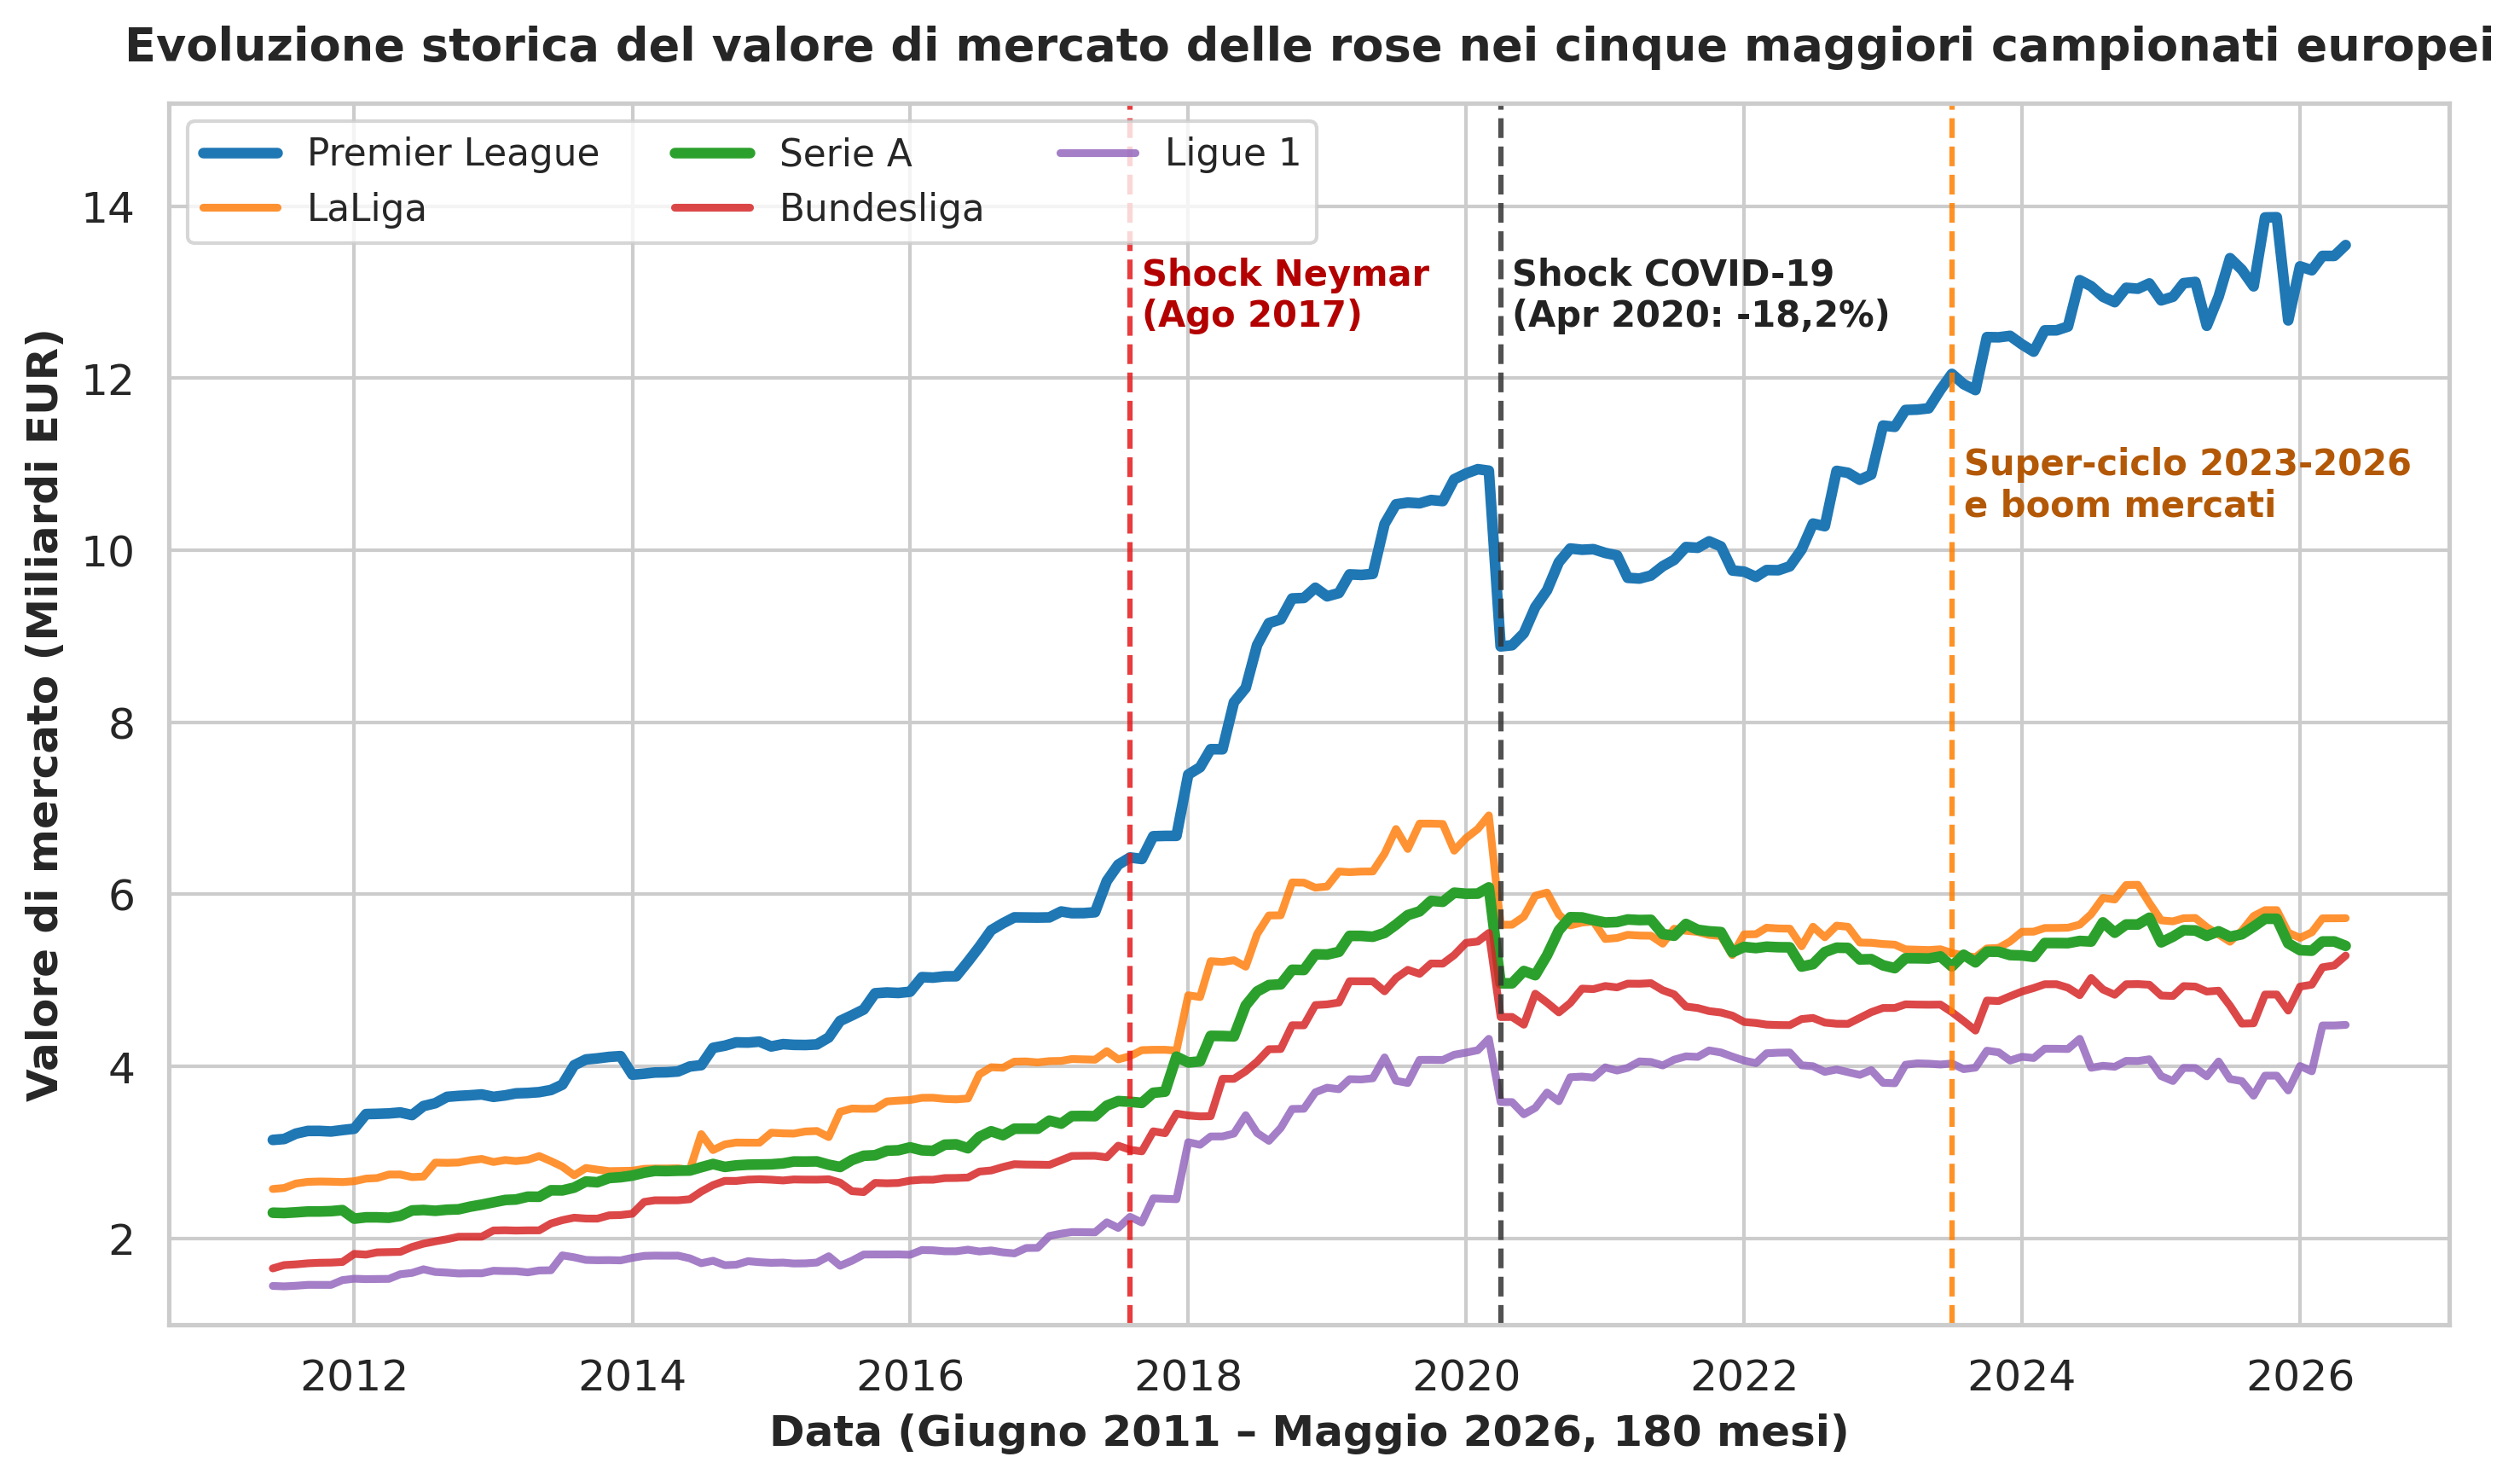
\includegraphics[width=0.95\textwidth]{capitolo7/img/fig03_eda_valore_campionati.png}
    \caption{Evoluzione storica del valore di mercato delle rose nei cinque maggiori campionati europei tra giugno 2011 e maggio 2026.}
    \label{fig:eda_valore_campionati}
\end{figure}

Come emerge con chiarezza dalla Figura \ref{fig:eda_valore_campionati} e dal confronto quantitativo riportato nella Tabella \ref{tab:confronto_leghe_shock}, all'inizio della finestra di analisi (\texttt{2011-06}) il mercato calcistico europeo presentava un assetto relativamente bilanciato: la Premier League deteneva un valore complessivo di 3,15 miliardi di euro, seguita a breve distanza da LaLiga spagnola con 2,58 miliardi e dalla Serie A italiana con 2,30 miliardi, mentre la Bundesliga tedesca (1,65 miliardi) e la Ligue 1 francese (1,45 miliardi) completavano il perimetro dei cinque tornei.

\begin{table}[H]
\centering
\caption{Confronto del valore di mercato delle rose (in miliardi di euro) e delle variazioni percentuali nei cinque campionati europei attraverso le date chiave della serie storica.}
\label{tab:confronto_leghe_shock}
\begin{tabularx}{\textwidth}{lXXXXXXX}
\toprule
\textbf{Campionato} & \textbf{Giu 11} & \textbf{Lug 17} & \textbf{Mar 20} & \textbf{Apr 20} & \textbf{Mag 26} & \textbf{$\Delta\%$ COVID} & \textbf{$\Delta\%$ 15 anni} \\
\midrule
Premier League (\texttt{GB1}) & 3,15 & 6,35 & 10,92 & 8,88 & 13,55 & $-18,70\%$ & $+330,6\%$ \\
LaLiga (\texttt{ES1}) & 2,58 & 4,08 & 6,92 & 5,65 & 5,72 & $-18,36\%$ & $+122,2\%$ \\
Serie A (\texttt{IT1}) & 2,30 & 3,60 & 6,08 & 4,97 & 5,40 & $-18,34\%$ & $+134,9\%$ \\
Bundesliga (\texttt{L1}) & 1,65 & 3,08 & 5,55 & 4,57 & 5,29 & $-17,60\%$ & $+220,0\%$ \\
Ligue 1 (\texttt{FR1}) & 1,45 & 2,12 & 4,32 & 3,59 & 4,48 & $-17,01\%$ & $+209,4\%$ \\
\midrule
\textbf{Totale Top-5} & \textbf{11,12} & \textbf{19,23} & \textbf{33,79} & \textbf{27,65} & \textbf{34,44} & \textbf{$-18,17\%$} & \textbf{$+209,7\%$} \\
\bottomrule
\end{tabularx}
\end{table}

La progressiva trasformazione dei rapporti di forza è resa evidente dalla dinamica delle quote percentuali sul totale continentale (\textit{Market Share \%}), rappresentata mediante area cumulativa nella Figura \ref{fig:eda_quote_mercato}.

\begin{figure}[H]
    \centering
    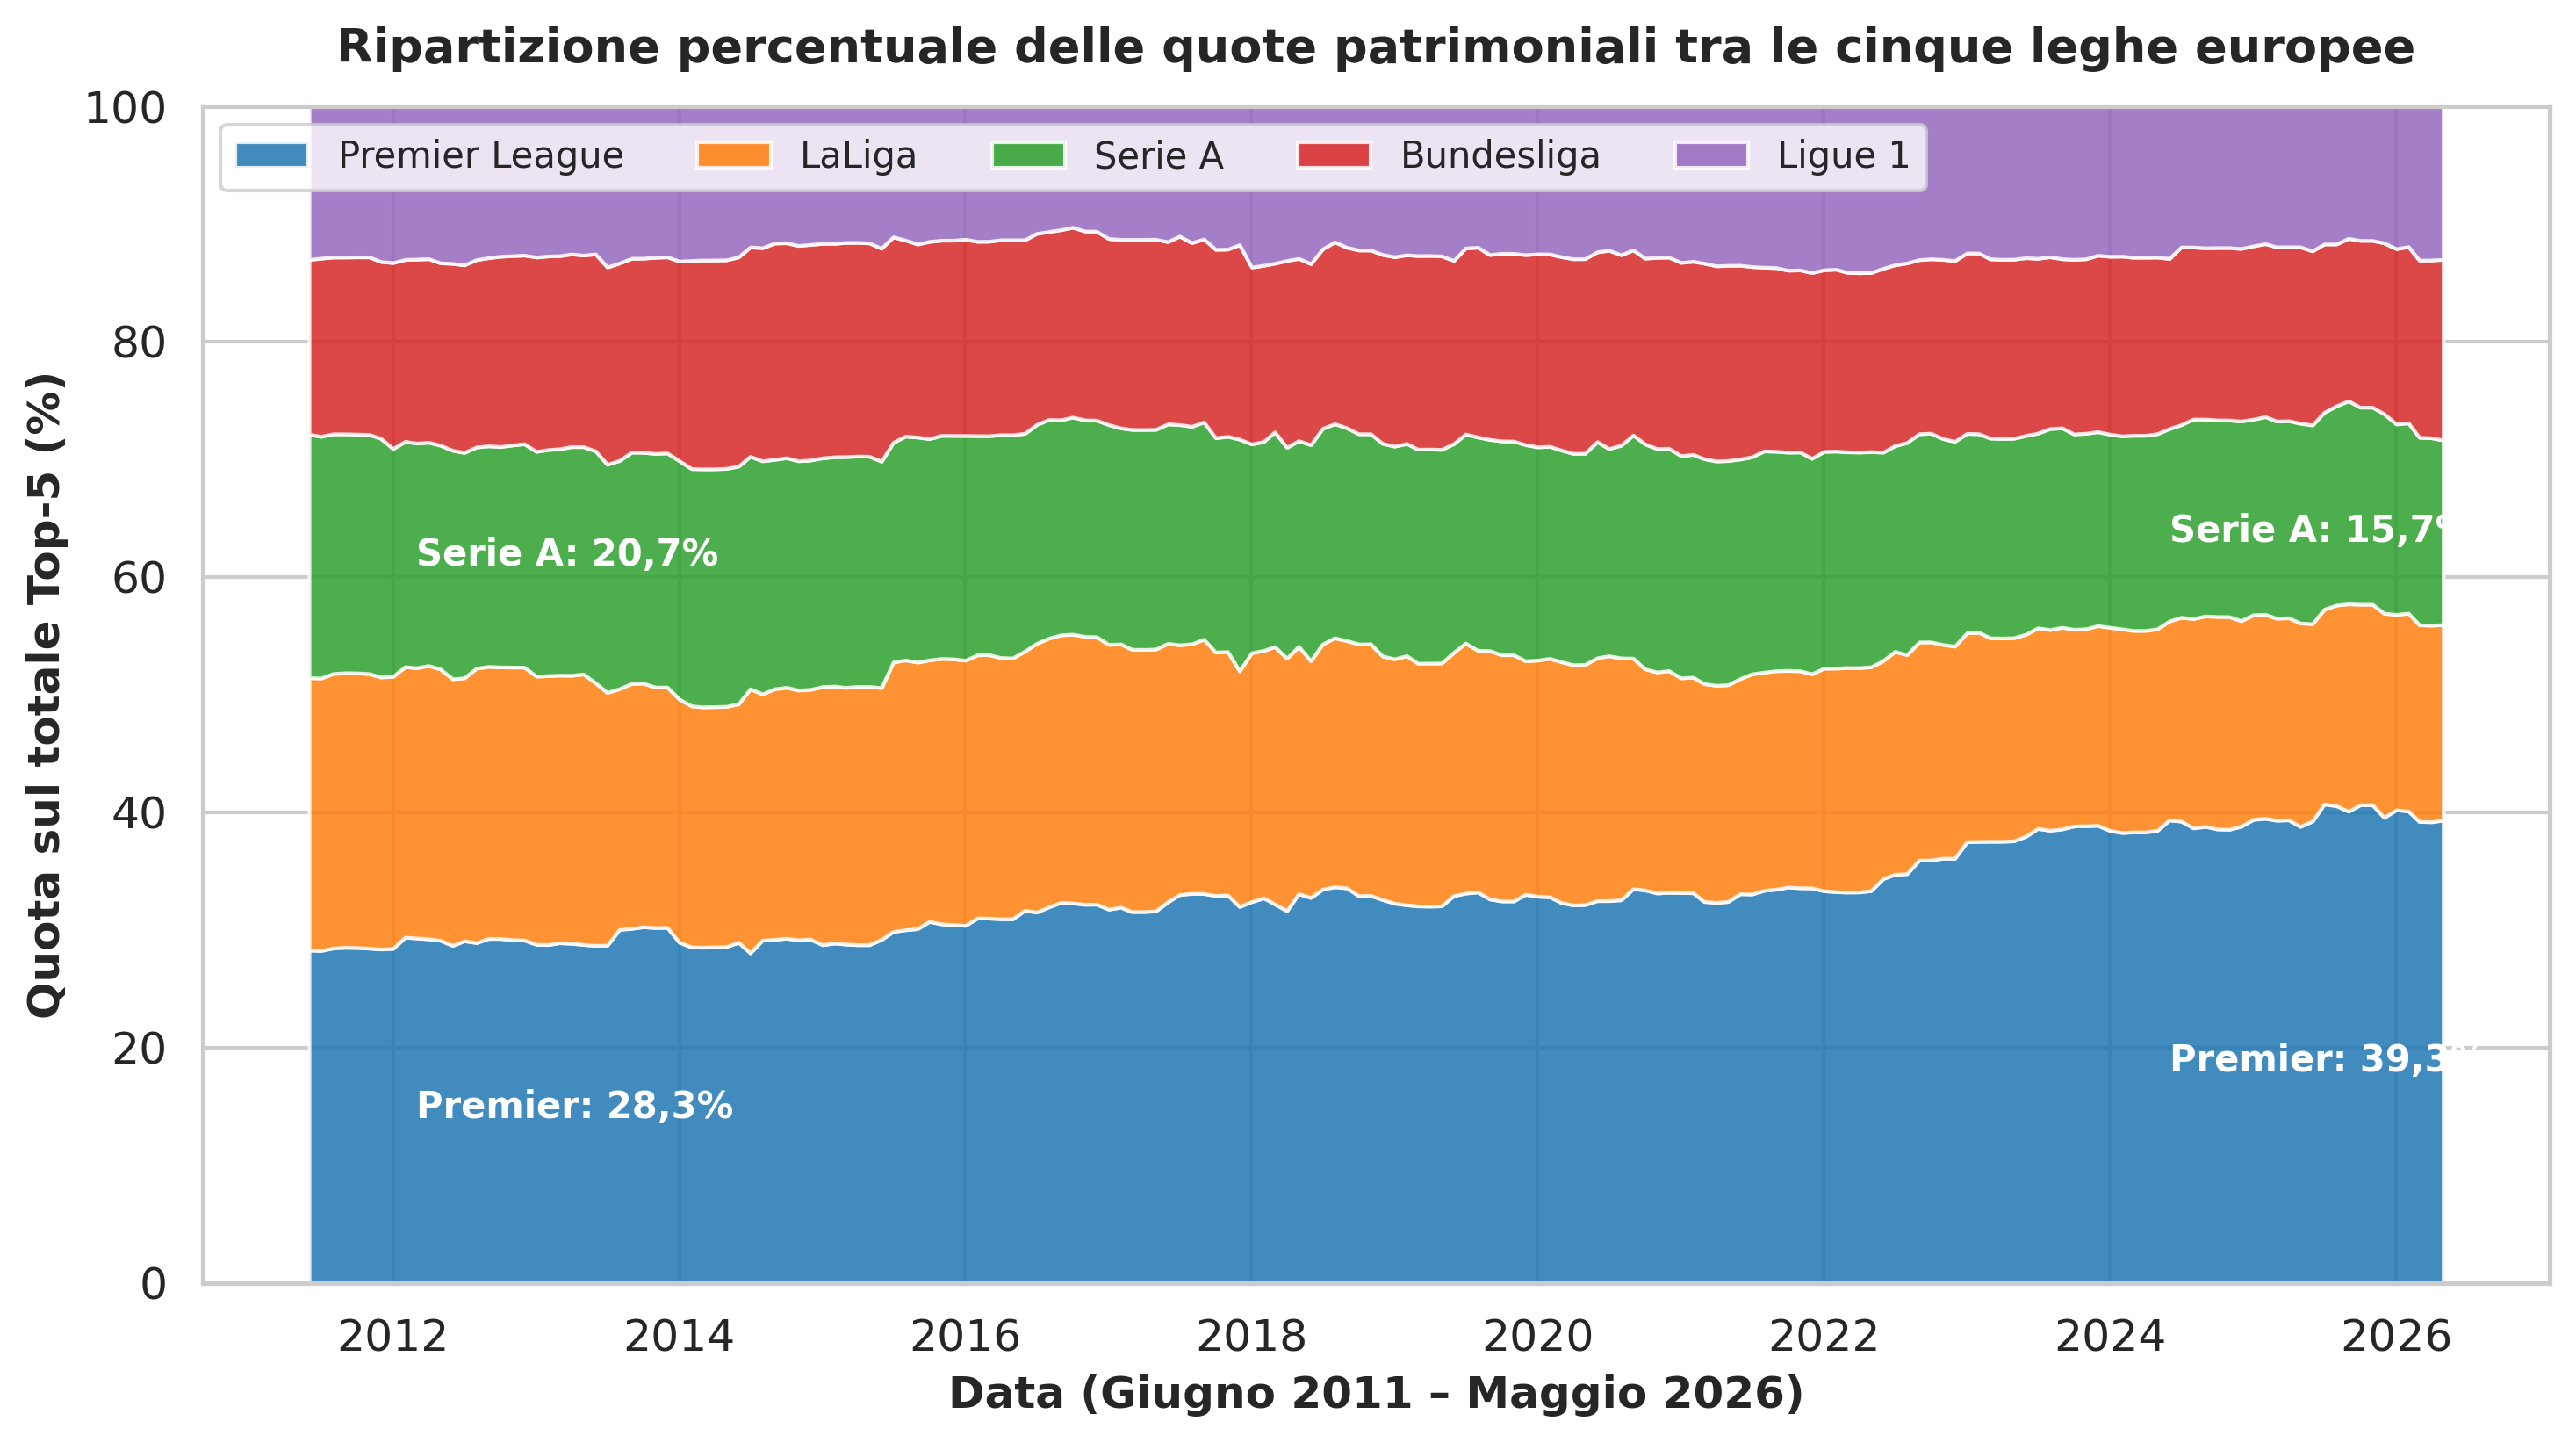
\includegraphics[width=0.95\textwidth]{capitolo7/img/fig04_eda_quote_mercato.png}
    \caption{Ripartizione percentuale delle quote patrimoniali tra le cinque leghe europee sul totale Top-5 (2011–2026).}
    \label{fig:eda_quote_mercato}
\end{figure}

Lungo i quindici anni successivi, la superiore capacità commerciale della lega inglese nella negoziazione dei diritti televisivi ha scavato un solco incolmabile: tra il 2011 e il 2026 la Premier League è cresciuta del 330,6\%, toccando un massimo assoluto di 13,87 miliardi di euro nel novembre 2025 e chiudendo a 13,55 miliardi nel maggio 2026, data in cui assorbe da sola il 39,3\% dell'intero patrimonio calcistico europeo dei Top-5 campionati (Figura \ref{fig:eda_quote_mercato}).

La Serie A italiana (\texttt{serie\_a\_market\_value\_bn}) ha invece attraversato tre fasi distinte. Nel quinquennio 2011--2015 il campionato italiano ha conosciuto una fase di sostanziale stasi, salendo lentamente da 2,30 a 2,90 miliardi di euro. Tra il 2016 e l'inizio del 2020, spinta da ingenti investimenti, la Serie A ha accelerato toccando il massimo storico di 6,08 miliardi di euro nel marzo 2020. Dopo il violento crollo pandemico, la risalita del torneo italiano si è assestata su ritmi più contenuti rispetto all'Inghilterra: nel maggio 2026 la Serie A si attesta a 5,40 miliardi di euro (quota del 15,7\% sul totale Top-5 e crescita complessiva del 134,9\%), collocandosi al terzo posto alle spalle de LaLiga (5,72 miliardi, 16,6\%) e di poco sopra alla Bundesliga (5,29 miliardi, 15,4\%).

\subsection{Anatomia dei tre shock storici: inflazione del 2017, crollo COVID-19 e ciclo post-2023}

Uno degli esiti più significativi dell'analisi della serie storica è l'individuazione di tre brusche discontinuità strutturali ben delimitate nel tempo, le quali violano l'ipotesi di crescita stazionaria uniforme e impongono l'uso di variabili indicatrici d'intervento nella modellazione predittiva.

Il primo shock strutturale coincide con l'agosto 2017 (\texttt{2017-08}), data del trasferimento record di Neymar dal Barcellona al Paris Saint-Germain per 222 milioni di euro e del rinnovo dei diritti TV internazionali. Come visualizzato nel dettaglio della Figura \ref{fig:eda_shock_neymar}, questo evento ha prodotto un immediato cambio di pendenza (\textit{slope change}) del trend economico: mentre tra giugno 2011 e luglio 2017 la serie aggregata europea cresceva a un ritmo di $+1,31$ miliardi di euro all'anno, nei trentadue mesi successivi ad agosto 2017 la crescita annualizzata è quadruplicata, toccando un tasso di $+5,46$ miliardi di euro all'anno.

\begin{figure}[H]
    \centering
    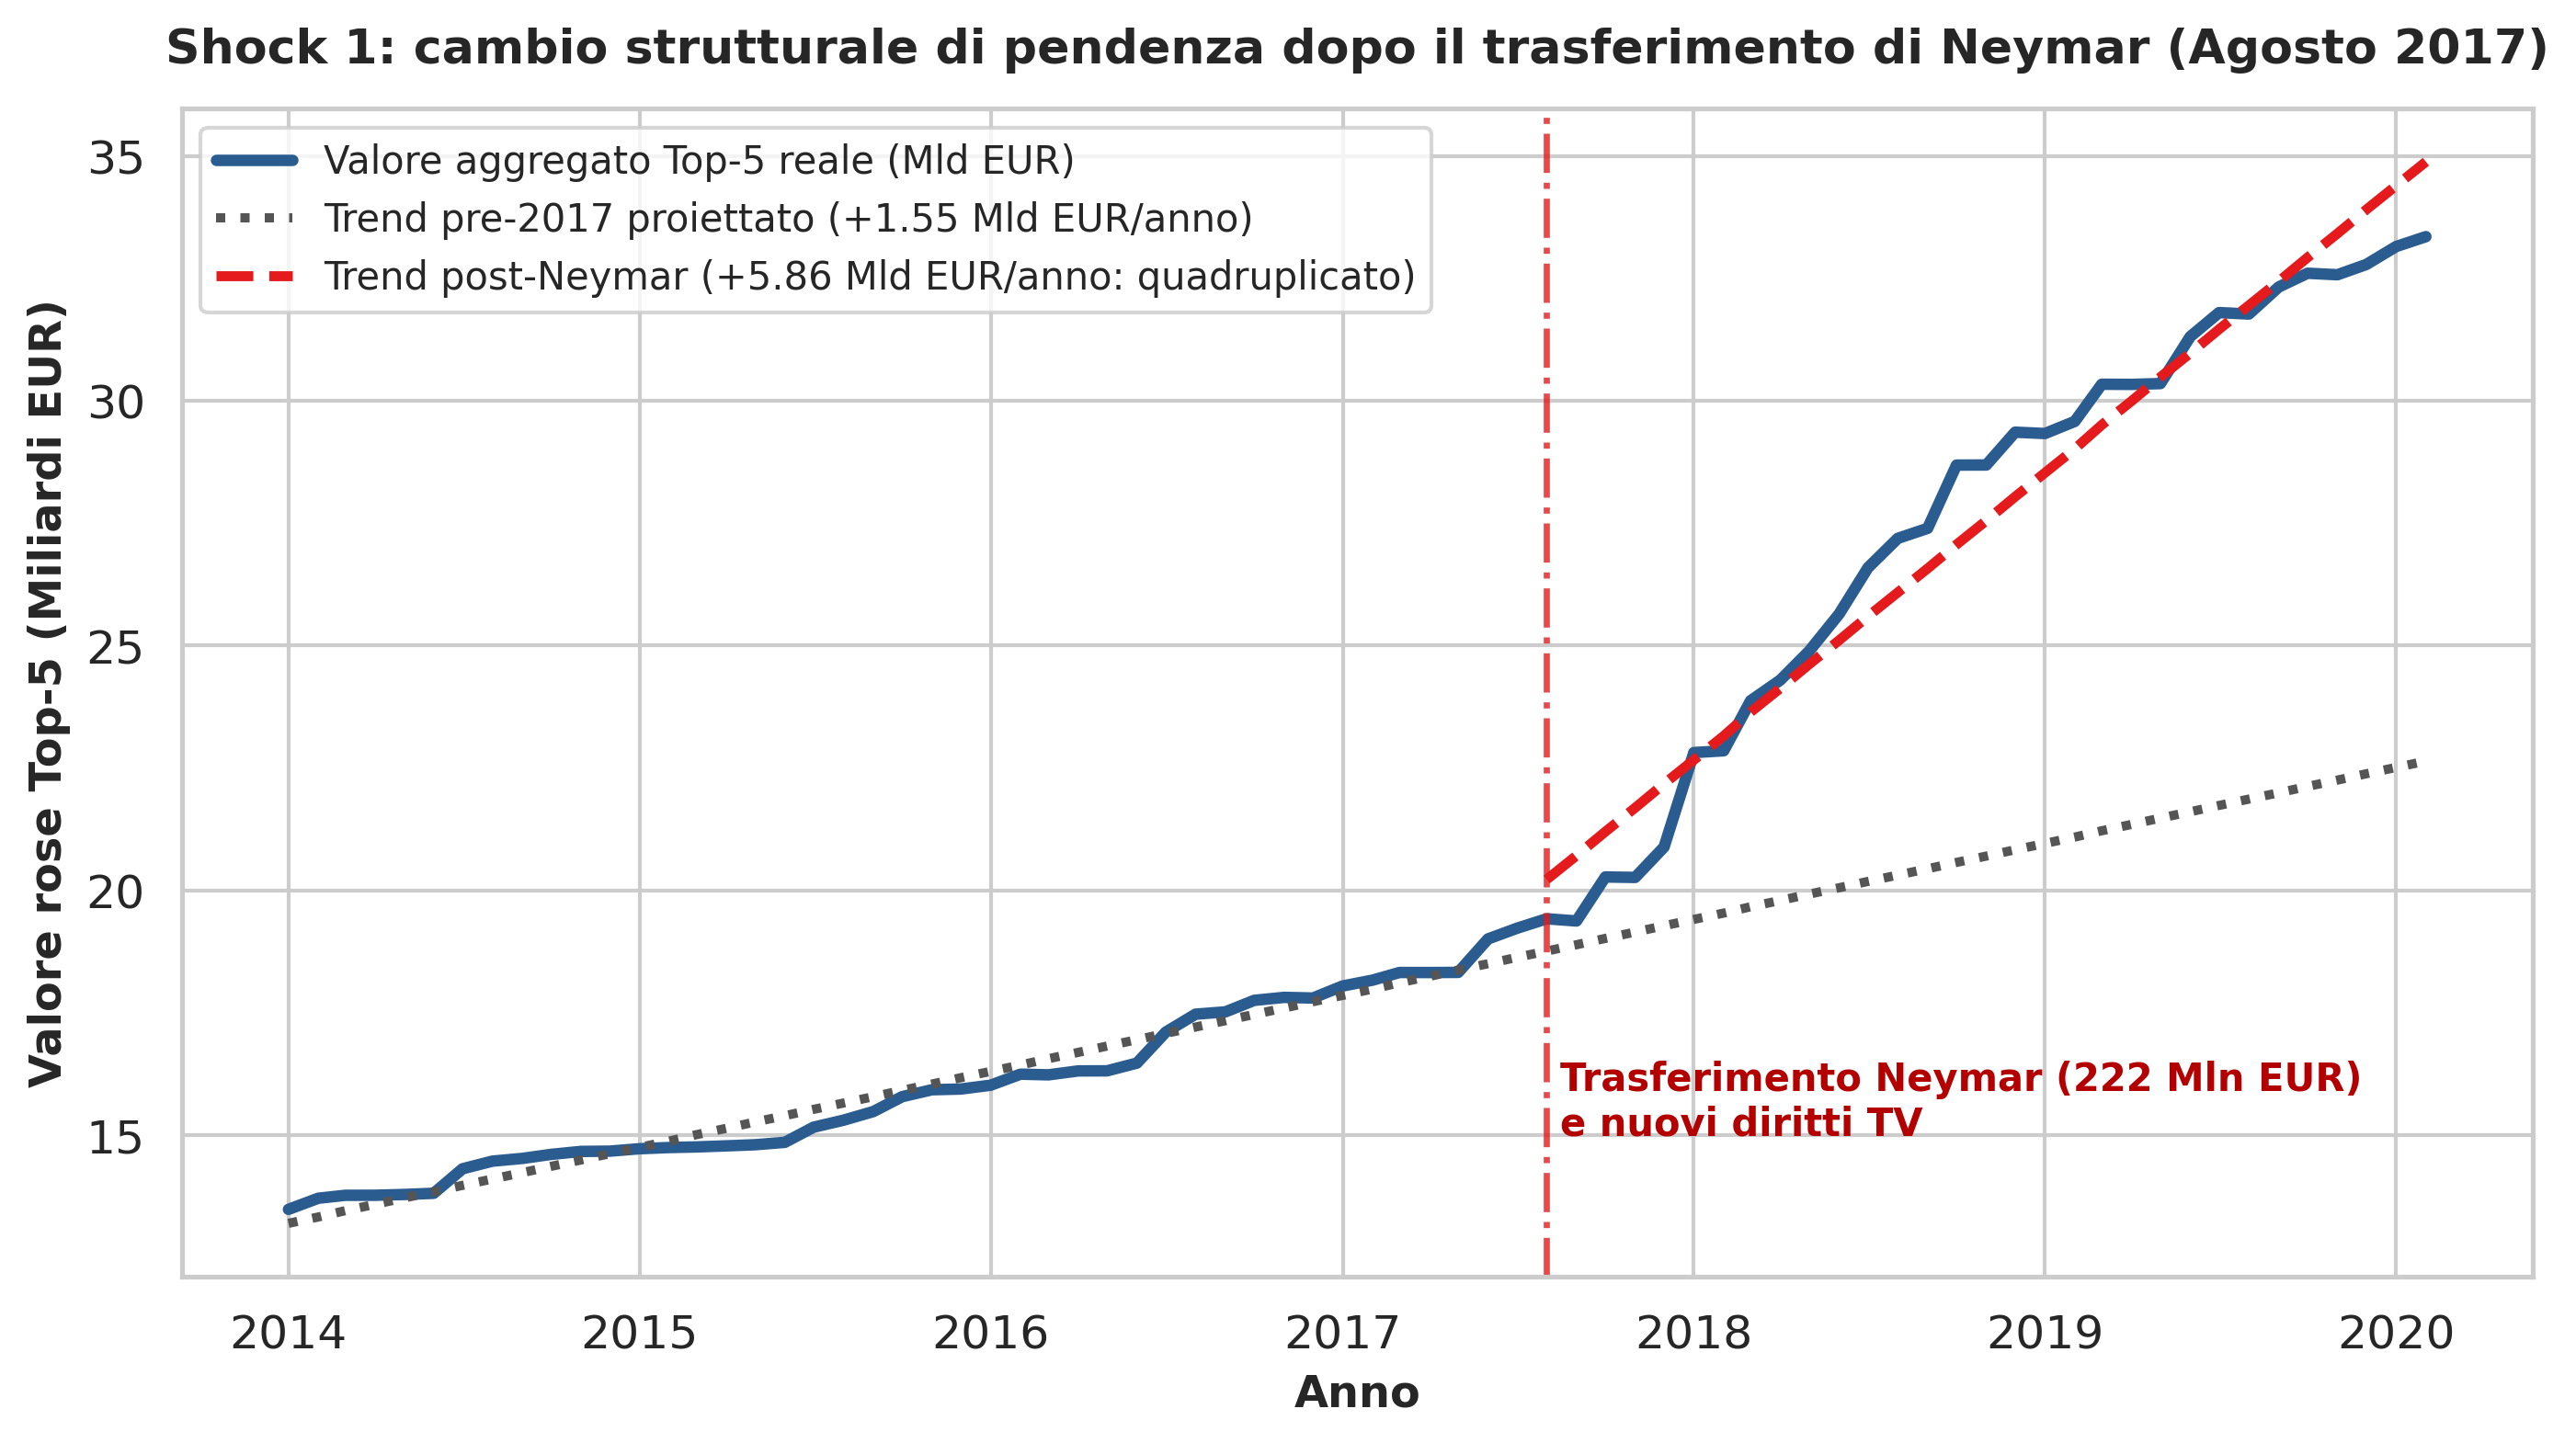
\includegraphics[width=0.92\textwidth]{capitolo7/img/fig05_eda_shock_neymar_2017.png}
    \caption{Shock 1: cambio strutturale di pendenza nel trend del valore aggregato Top-5 a seguito del trasferimento di Neymar nell'agosto 2017.}
    \label{fig:eda_shock_neymar}
\end{figure}

Il secondo shock, illustrato nella Figura \ref{fig:eda_shock_covid}, rappresenta il più drammatico evento di rottura nella storia economica del settore: l'esplosione della pandemia da COVID-19 e la sospensione totale delle competizioni sportive nella primavera del 2020. Di fronte al blocco dei ricavi da stadio e all'incertezza finanziaria, nell'aprile 2020 (\texttt{2020-04}) la piattaforma Transfermarkt ha applicato un taglio straordinario generalizzato, effettuando 4.379 ribassi di cartellino in trenta giorni. Tra marzo e aprile 2020 il valore europeo è crollato istantaneamente da 33,79 a 27,65 miliardi di euro ($-18,17\%$, con una perdita secca di 6,14 miliardi di euro), mentre la Serie A è precipitata da 6,08 a 4,97 miliardi ($-18,34\%$). Come evidenziato dalla linea tratteggiata del picco pre-pandemico, la serie ha impiegato esattamente 55 mesi (oltre quattro anni e mezzo) per ritornare ai livelli pre-crisi, superando nuovamente la soglia dei 33,79 miliardi solo nell'ottobre 2024 (33,83 miliardi di euro).

\begin{figure}[H]
    \centering
    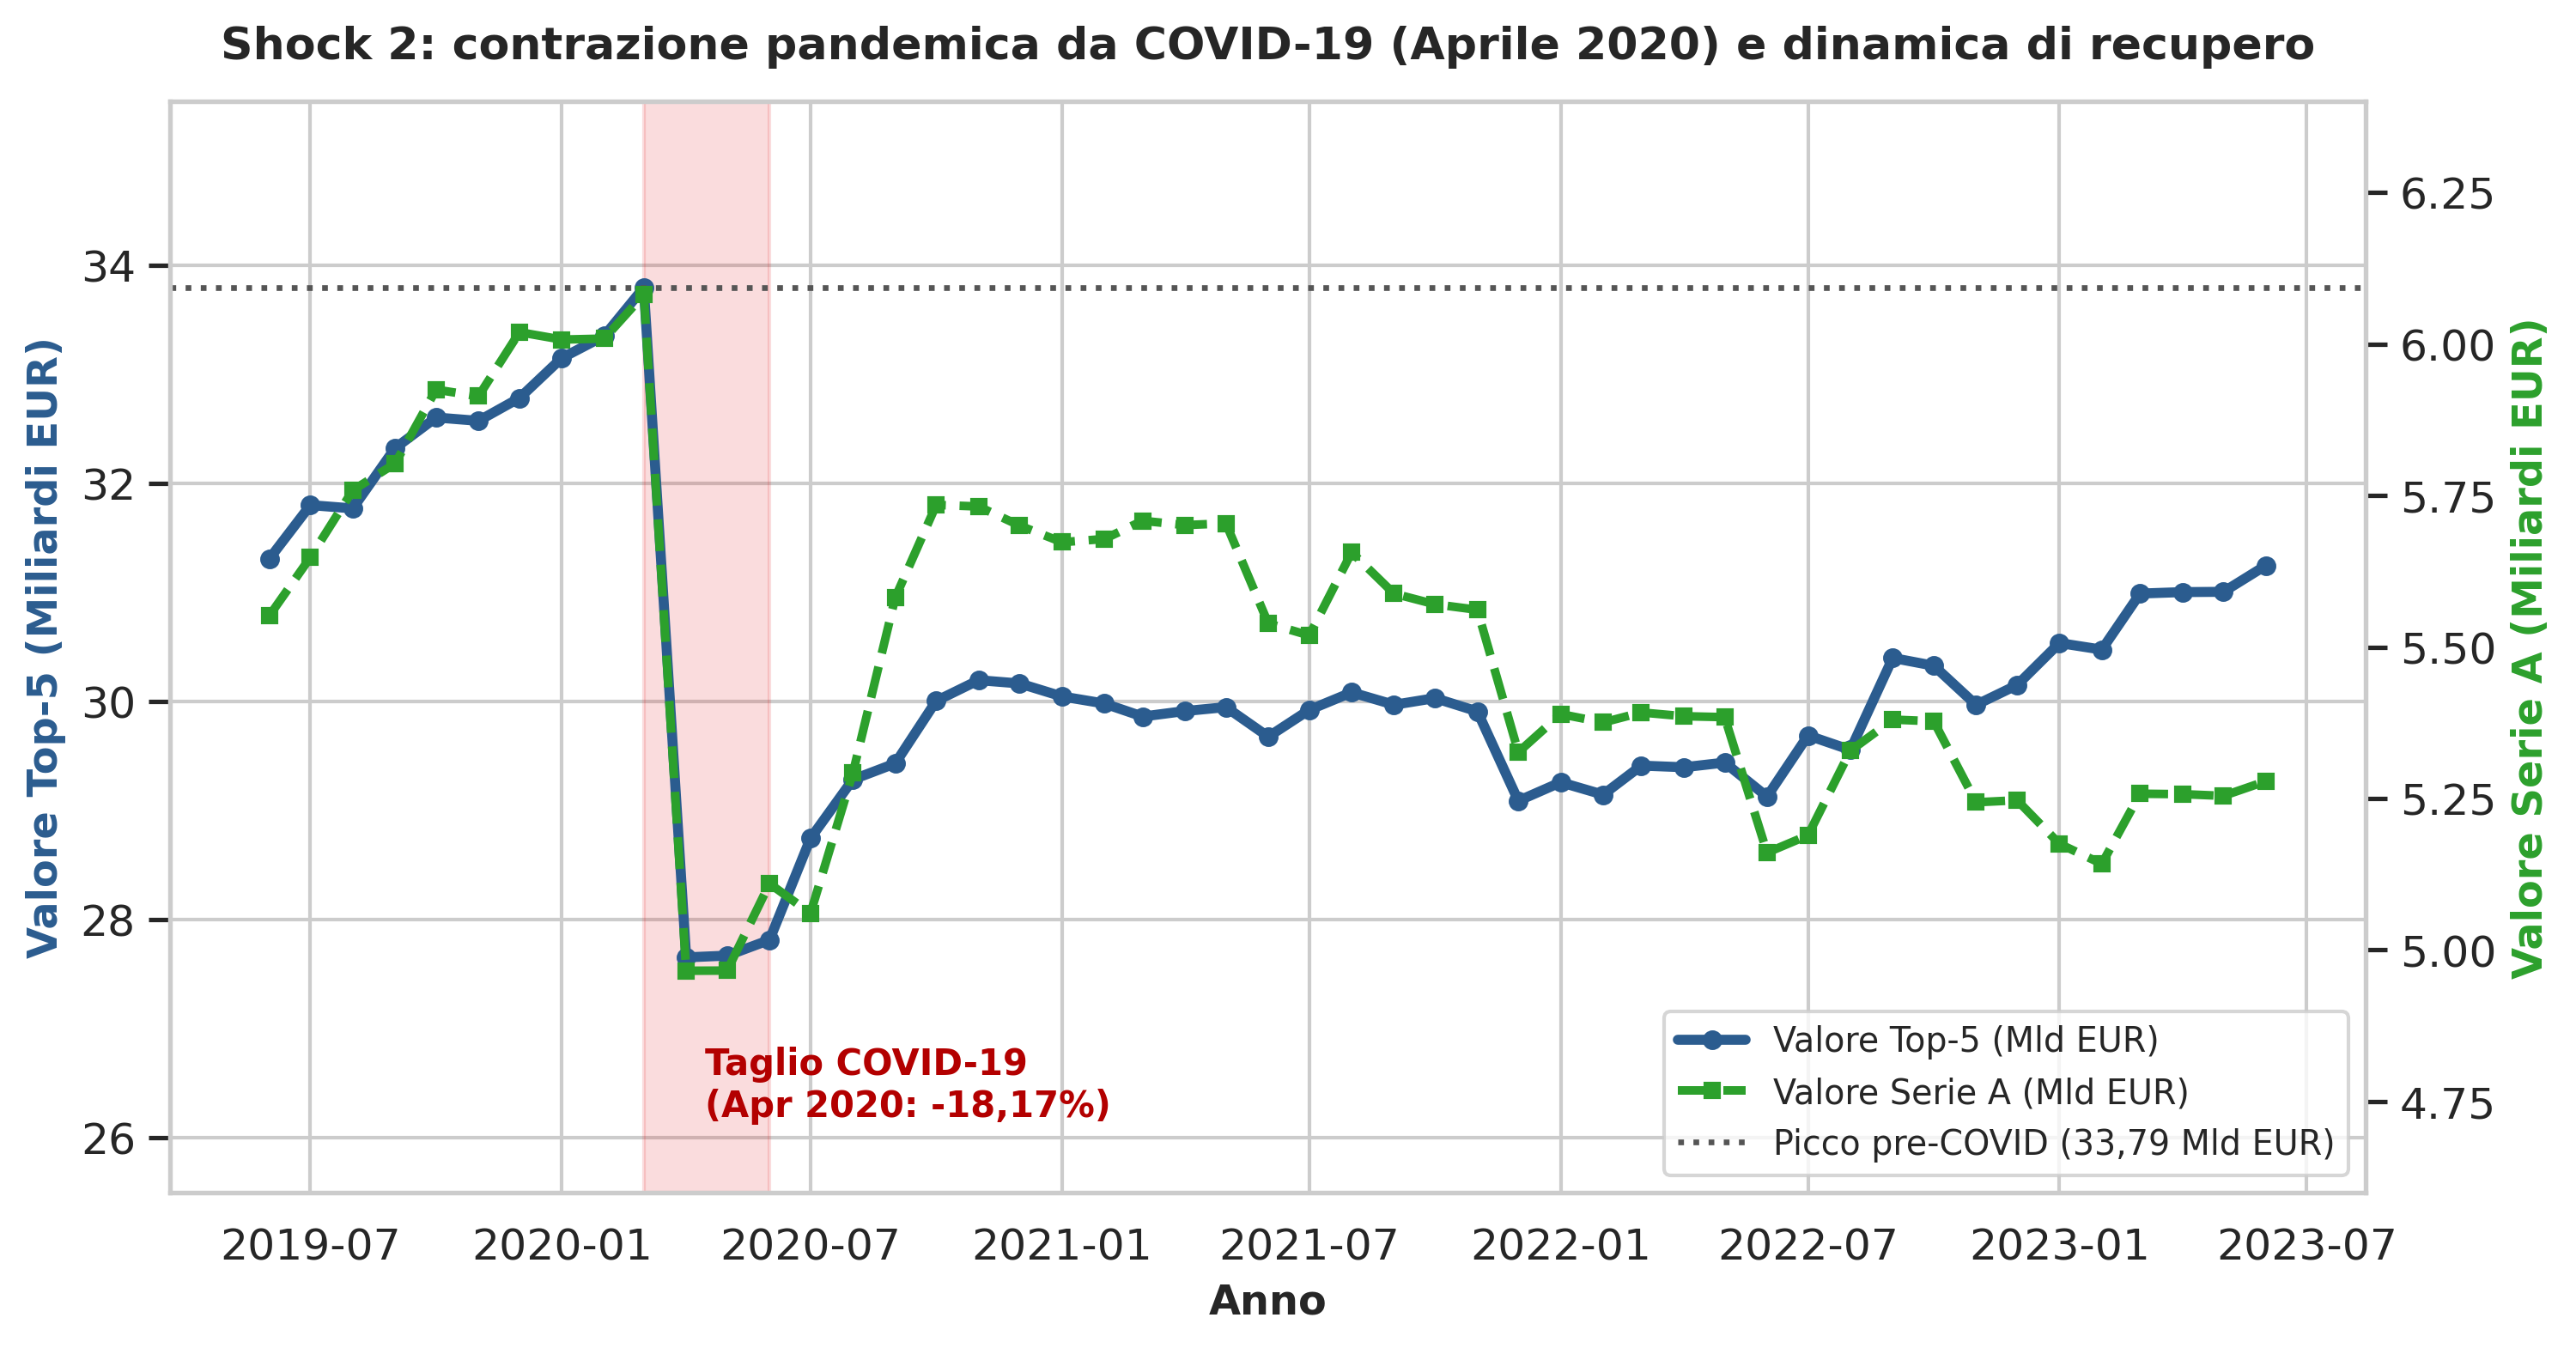
\includegraphics[width=0.92\textwidth]{capitolo7/img/fig06_eda_shock_covid_2020.png}
    \caption{Shock 2: contrazione pandemica da COVID-19 nell'aprile 2020 ($-18,17\%$) e dinamica temporale di recupero del valore patrimoniale.}
    \label{fig:eda_shock_covid}
\end{figure}

Il terzo fenomeno strutturale, mostrato nella Figura \ref{fig:eda_shock_boom}, descrive la forte ripartenza del triennio 2023--2026, sostenuta dall'irruzione finanziaria della Saudi Pro League nell'estate 2023 e dall'entrata in vigore del nuovo format allargato della UEFA Champions League a partire dalla stagione 2024/2025. Tale fase conduce la serie al massimo storico assoluto di 34,44 miliardi di euro nel maggio 2026 e si caratterizza per una massiccia rivalutazione dei cartellini dei calciatori di vertice: il valore medio per giocatore attivo (\texttt{mean\_player\_value\_m}), rimasto attorno ai 3 milioni di euro fino al 2017 e pari a 5,07 milioni nel marzo 2020, accelera fino a superare la soglia degli 11 milioni di euro (11,01 milioni) nella primavera del 2026.

\begin{figure}[H]
    \centering
    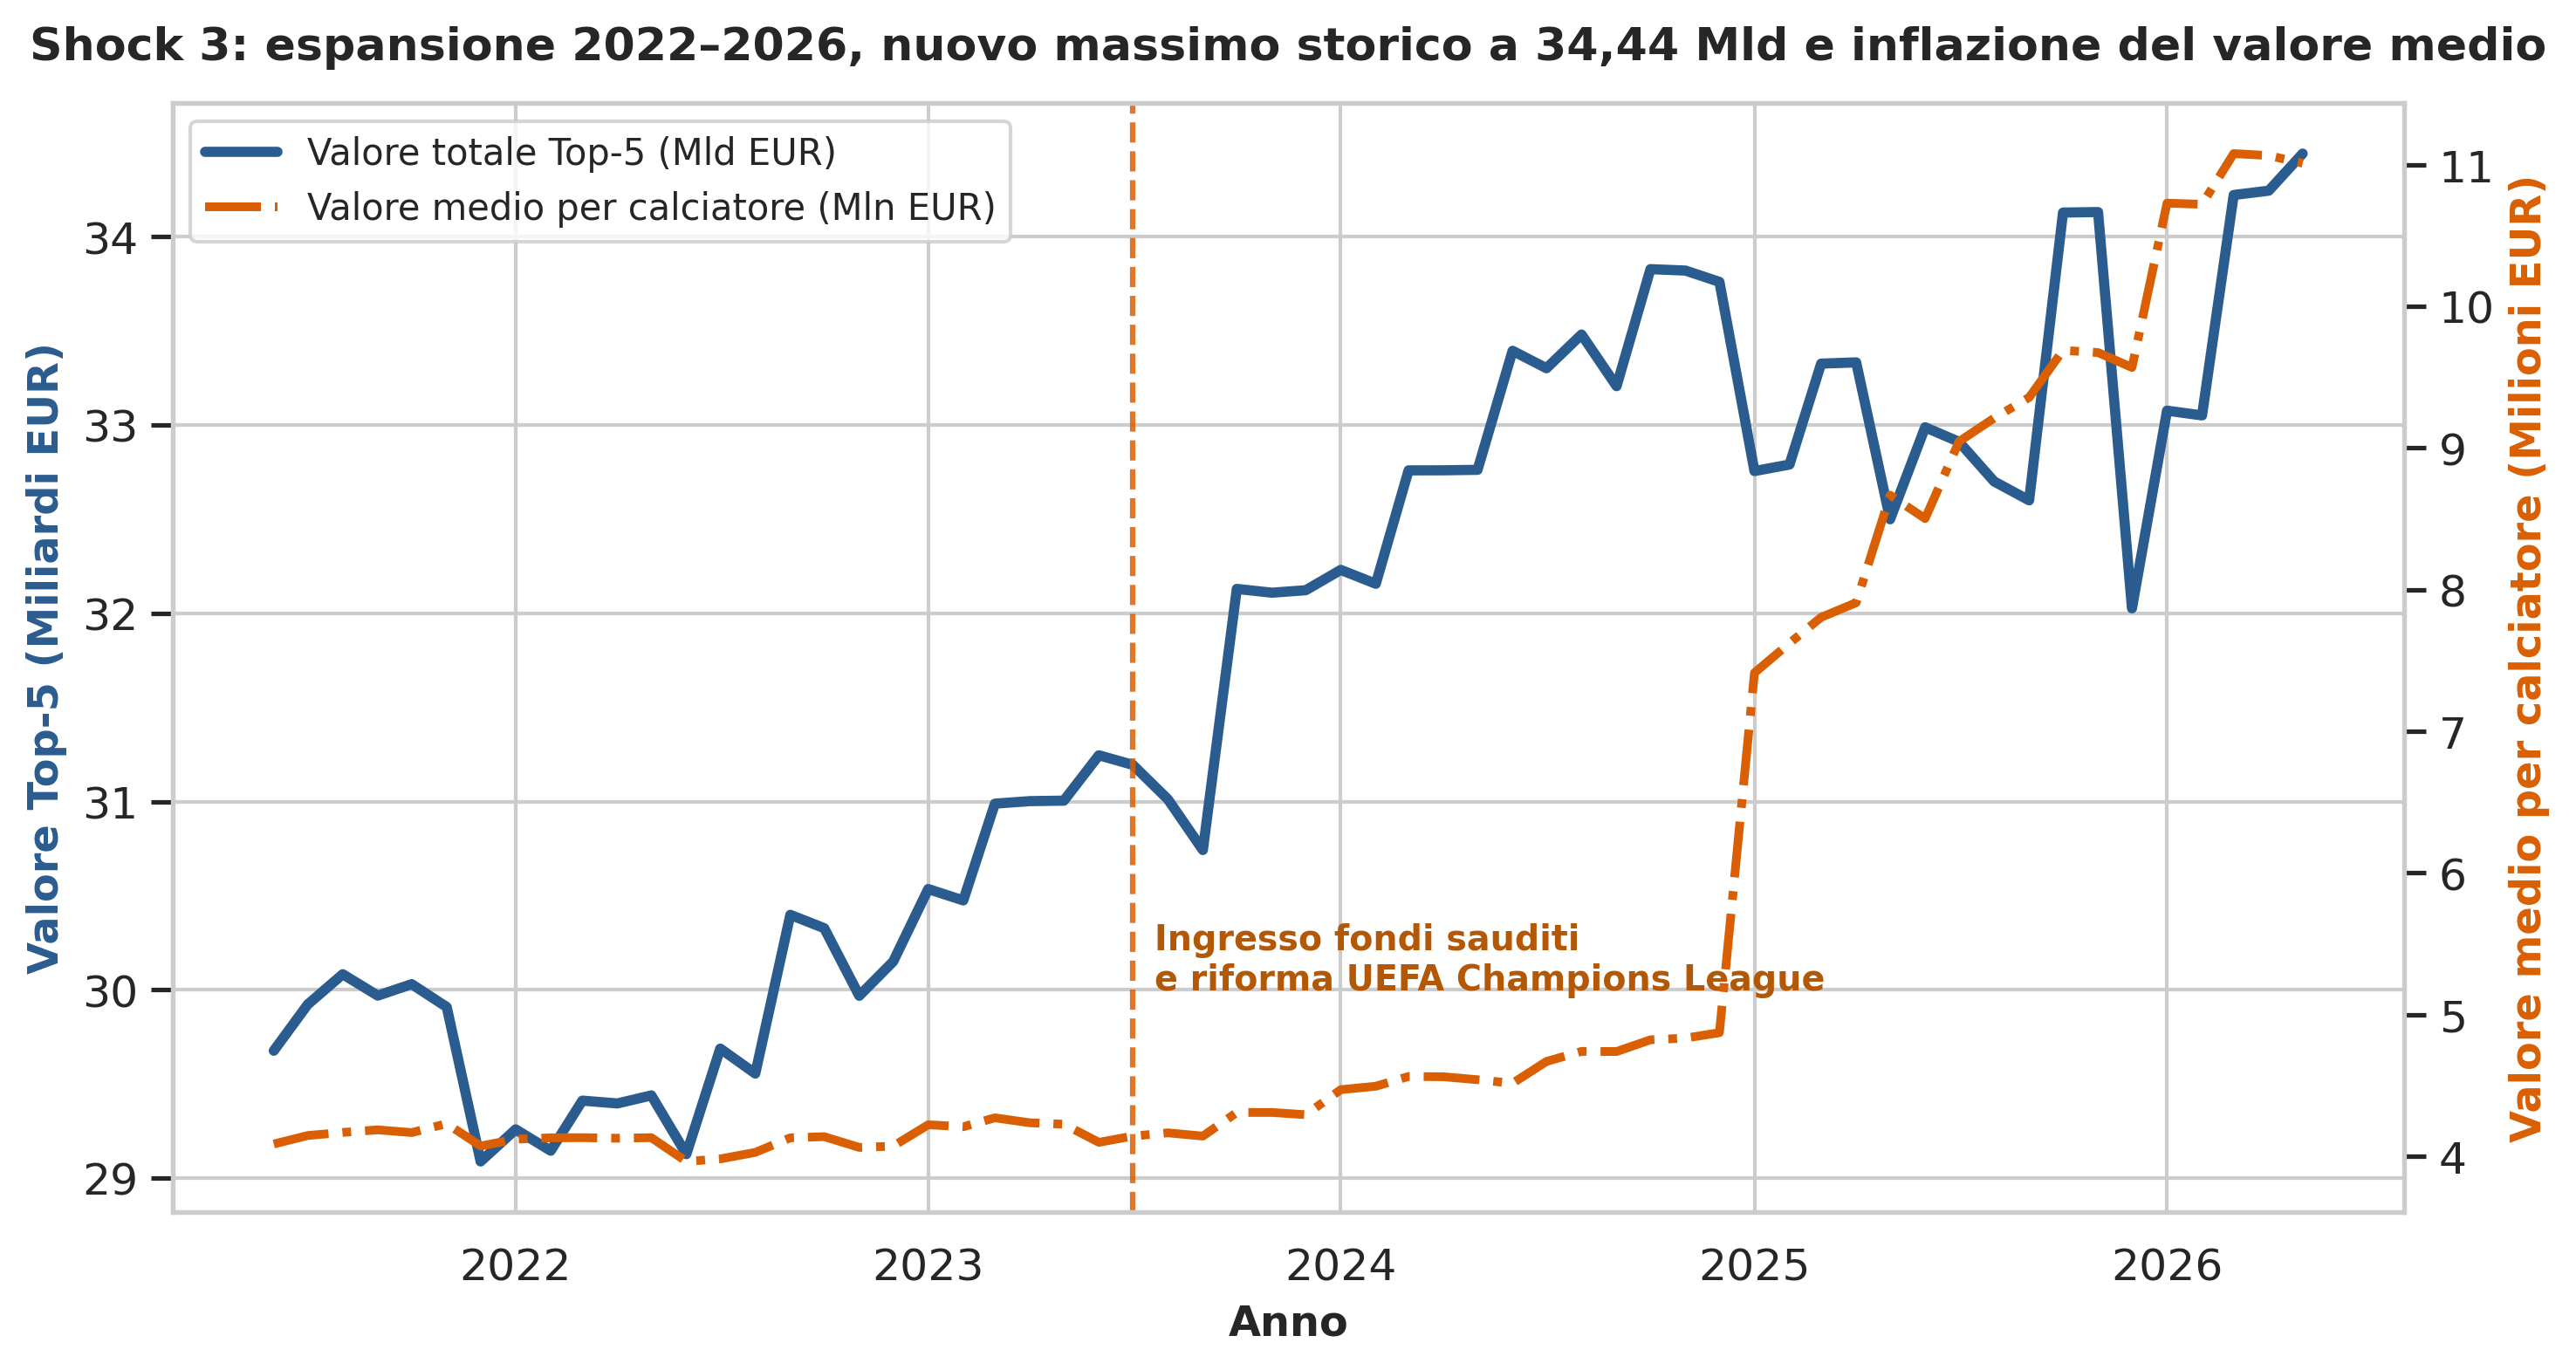
\includegraphics[width=0.92\textwidth]{capitolo7/img/fig07_eda_shock_boom_2026.png}
    \caption{Shock 3: espansione post-2023, nuovo massimo storico a 34,44 miliardi di euro e impennata del valore medio per giocatore.}
    \label{fig:eda_shock_boom}
\end{figure}

\subsection{Analisi delle variazioni percentuali mensili, volatilità e identificazione degli outlier}

Per analizzare il comportamento dinamico della serie al netto del trend di fondo, è stata calcolata la serie delle variazioni percentuali mensili (\textit{Change \%}):
\begin{equation}
    \Delta\%_t = \frac{Y_t - Y_{t-1}}{Y_{t-1}} \cdot 100
    \label{eq:pct_change}
\end{equation}
dove $Y_t$ indica il valore aggregato al mese $t$. Nella Figura \ref{fig:eda_change_pct} viene riportato l'andamento nel tempo di $\Delta\%_t$ con l'evidenziazione delle bande di variabilità naturale $\mu \pm 2\sigma$.

\begin{figure}[H]
    \centering
    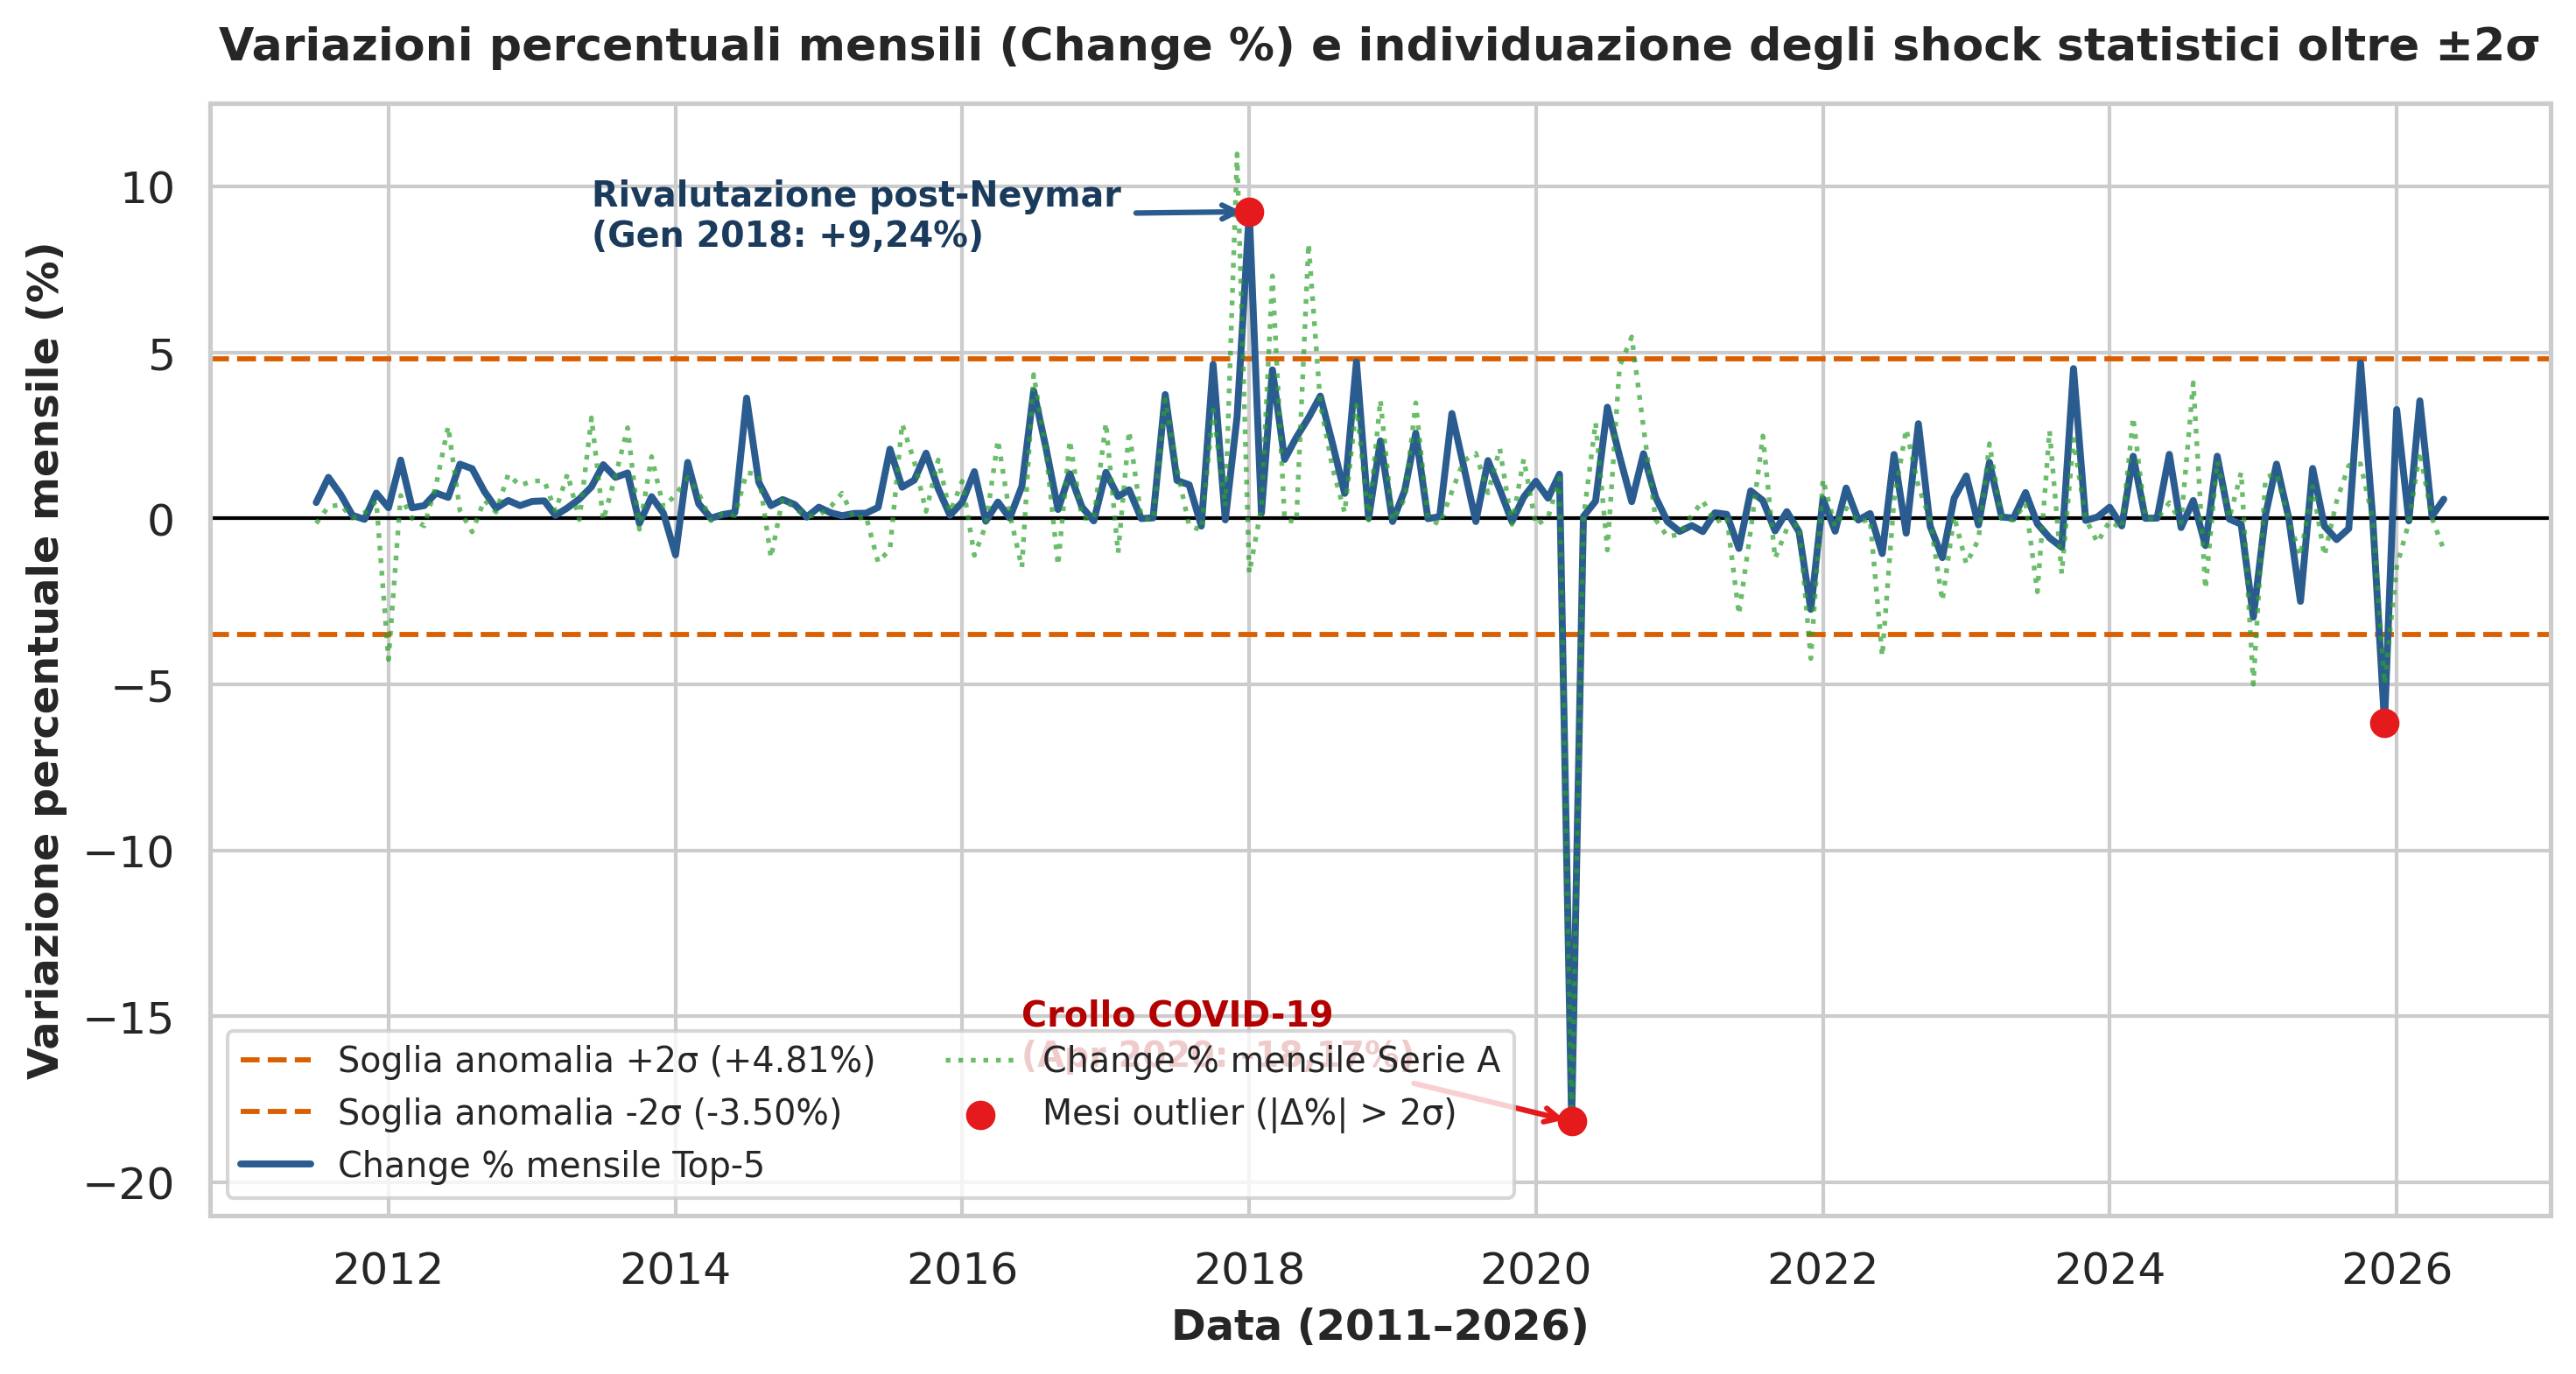
\includegraphics[width=0.95\textwidth]{capitolo7/img/fig08_eda_change_pct_volatilita.png}
    \caption{Serie storica delle variazioni percentuali mensili con fasce di confidenza $\pm 2\sigma$ e identificazione dei punti anomali.}
    \label{fig:eda_change_pct}
\end{figure}

Sull'arco delle 179 variazioni mensili tra luglio 2011 e maggio 2026, la variazione media mensile si attesta a $\mu = +0,66\%$ con una deviazione standard pari a $\sigma = 2,06\%$, definendo una fascia tipica $[\mu - 2\sigma, \, \mu + 2\sigma]$ compresa tra $-3,46\%$ e $+4,78\%$. Come visibile nella Figura \ref{fig:eda_change_pct}, l'applicazione del criterio $| \Delta\%_t - \mu | > 2\sigma$ permette di isolare con rigore statistico gli shock esogeni: il picco massimo si colloca nel gennaio 2018 ($+9,24\%$, a seguito dell'adeguamento generale dei listini post-Neymar), mentre il valore minimo coincide con il crollo pandemico di aprile 2020 ($-18,17\%$, un evento eccezionale a oltre nove deviazioni standard dalla media, $z = -9,14$).

La forma distributiva di tali variazioni è analizzata nella Figura \ref{fig:eda_distribuzione_kde} attraverso la stima di densità kernel (KDE).

\begin{figure}[H]
    \centering
    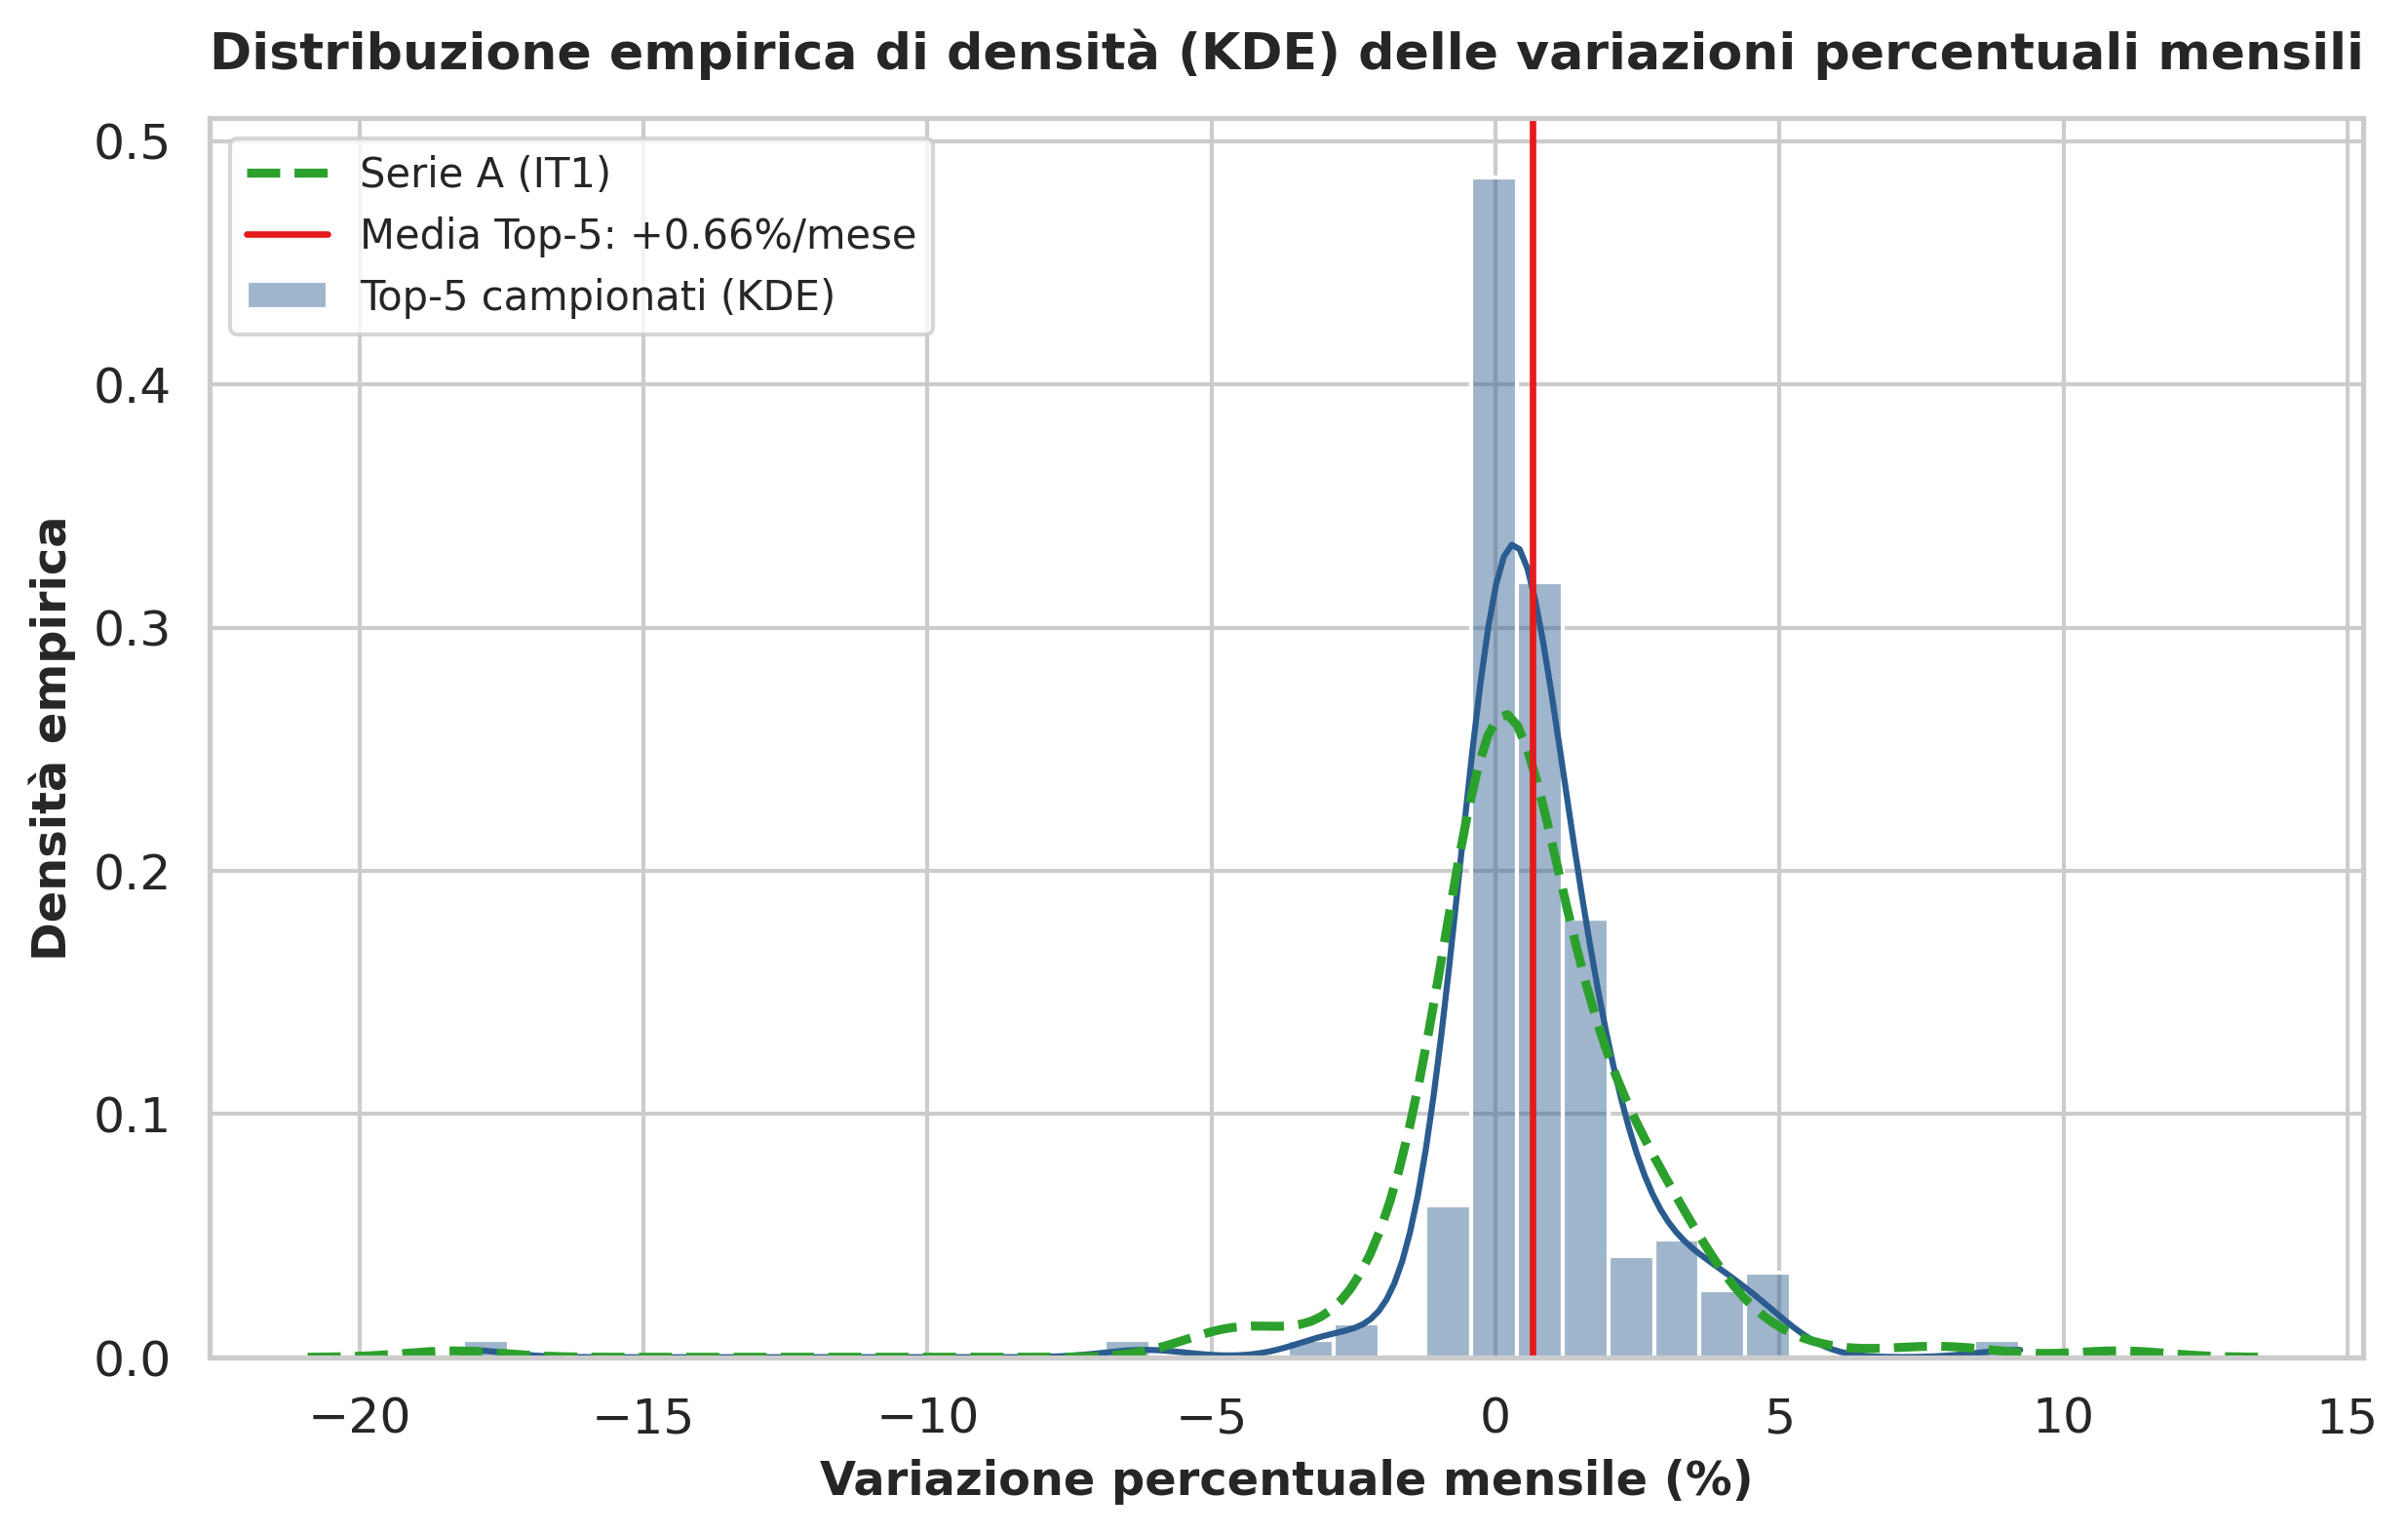
\includegraphics[width=0.88\textwidth]{capitolo7/img/fig09_eda_distribuzione_kde.png}
    \caption{Distribuzione empirica di densità (KDE) e istogramma delle variazioni percentuali mensili per i Top-5 campionati e la Serie A.}
    \label{fig:eda_distribuzione_kde}
\end{figure}

Come confermato dalla Figura \ref{fig:eda_distribuzione_kde}, la presenza di scossoni localizzati conferisce alla curva empirica una spiccata asimmetria negativa (\textit{skewness} pari a $-3,69$) e un'elevata curtosi (\textit{kurtosis} in eccesso pari a $35,48$, tipica di serie temporali con code pesanti e salti repentini). Inoltre, la Serie A (curva verde) manifesta una dispersione leggermente più ampia ($\sigma_{\text{IT1}} = 2,52\%$), dovuta al fatto che le contrattazioni e le rivalutazioni di una singola federazione nazionale risentono maggiormente della stagionalità del calendario rispetto all'aggregato europeo.

\subsection{Relazione dinamica tra valore delle rose e spese nelle sessioni di calciomercato}

L'ultimo asse d'indagine dell'analisi esplorativa studia il legame tra la serie di consistenza patrimoniale delle rose (\texttt{top5\_market\_value\_bn}) e i flussi monetari effettivi generati dal calciomercato (\texttt{transfer\_spend\_top5\_m}). Nel quindicennio considerato, i club delle cinque leghe hanno effettuato 31.000 trasferimenti in ingresso (di cui 8.105 a titolo oneroso), mobilitando una spesa cumulata di 65,82 miliardi di euro (di cui 14,68 miliardi spesi dalla sola Serie A, pari al 22,3\% del totale europeo).

Nella Figura \ref{fig:eda_spese_impulsi} viene confrontata la traiettoria del valore delle rose con gli impulsi mensili di spesa per trasferimenti.

\begin{figure}[H]
    \centering
    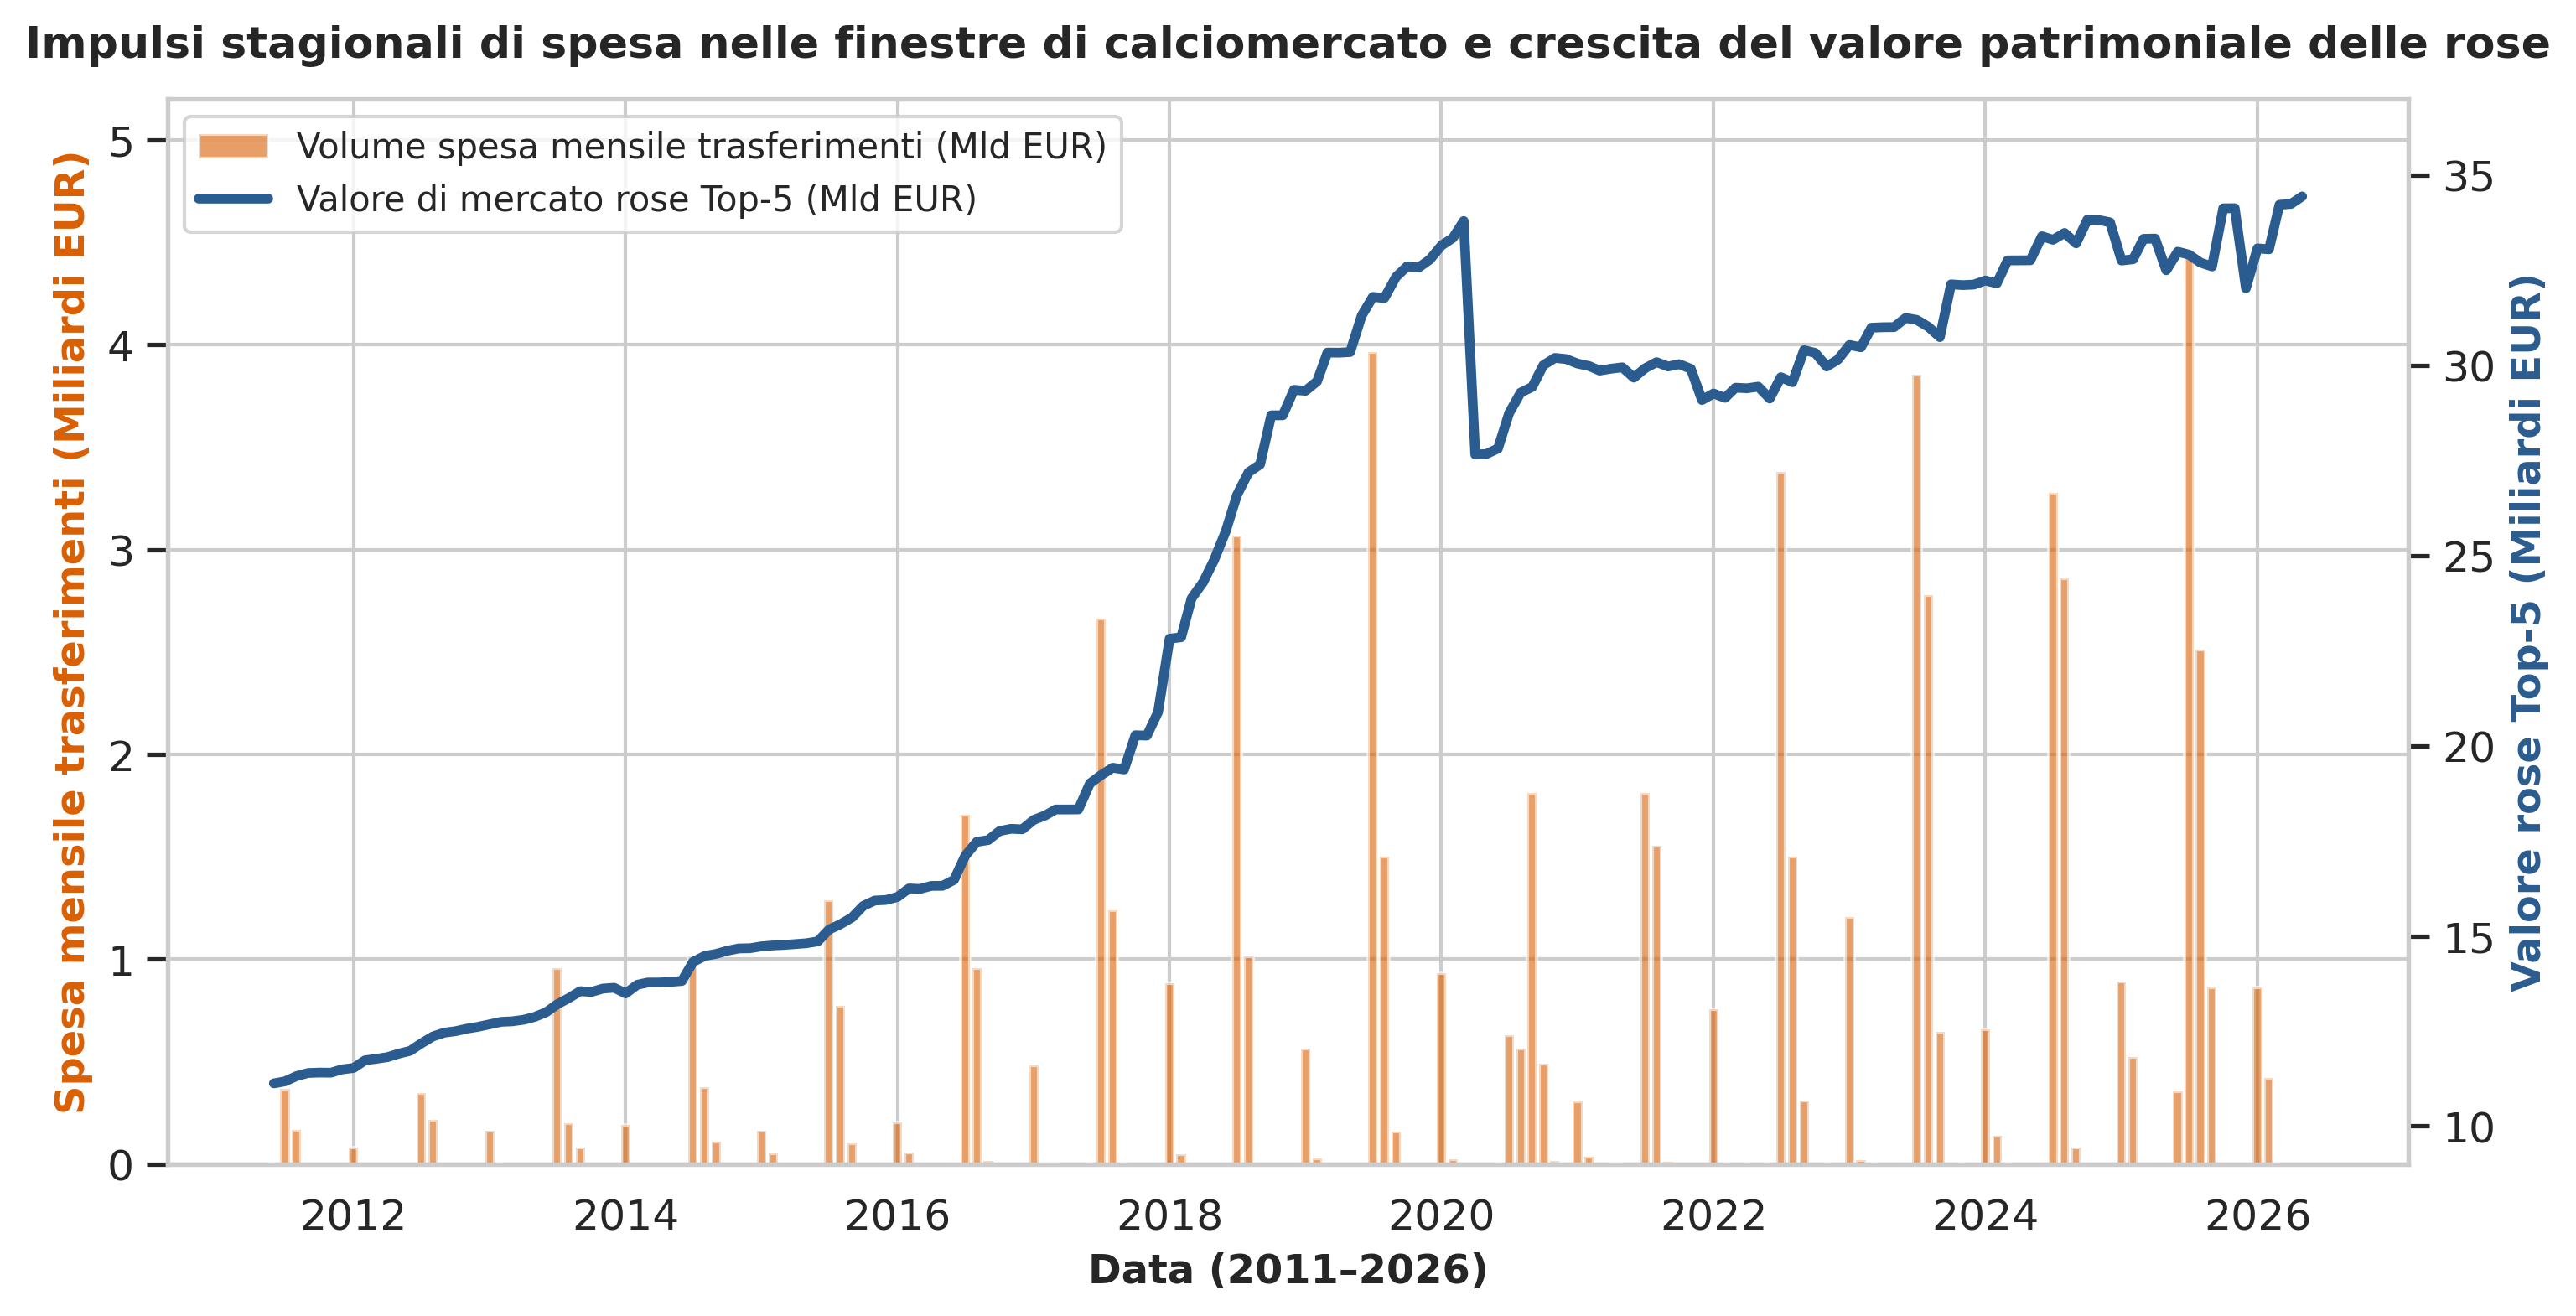
\includegraphics[width=0.95\textwidth]{capitolo7/img/fig10_eda_spese_calciomercato_impulsi.png}
    \caption{Impulsi stagionali di spesa nelle sessioni di calciomercato e crescita del valore patrimoniale delle rose (2011–2026).}
    \label{fig:eda_spese_impulsi}
\end{figure}

La Figura \ref{fig:eda_spese_impulsi} mette in risalto la marcata stagionalità della spesa per trasferimenti: i volumi monetari si concentrano quasi per intero nei mesi di luglio e agosto, con una finestra secondaria a gennaio, risultando quasi azzerati nei mesi restanti. Inoltre, l'altezza degli impulsi estivi cresce parallelamente all'espansione economica del settore: dai 533 milioni di euro dell'estate 2011 si giunge ai 3,90 miliardi dell'estate 2017 e ai 5,47 miliardi del 2019, fino a toccare il record assoluto nel luglio 2025 con 4.457,95 milioni di euro spesi in un solo mese (di cui 1.128,06 milioni in Serie A).

Per quantificare matematicamente la forza di questo legame, la Figura \ref{fig:eda_matrice_corr} riporta la matrice di correlazione lineare di Pearson tra le variabili patrimoniali e le grandezze di mercato.

\begin{figure}[H]
    \centering
    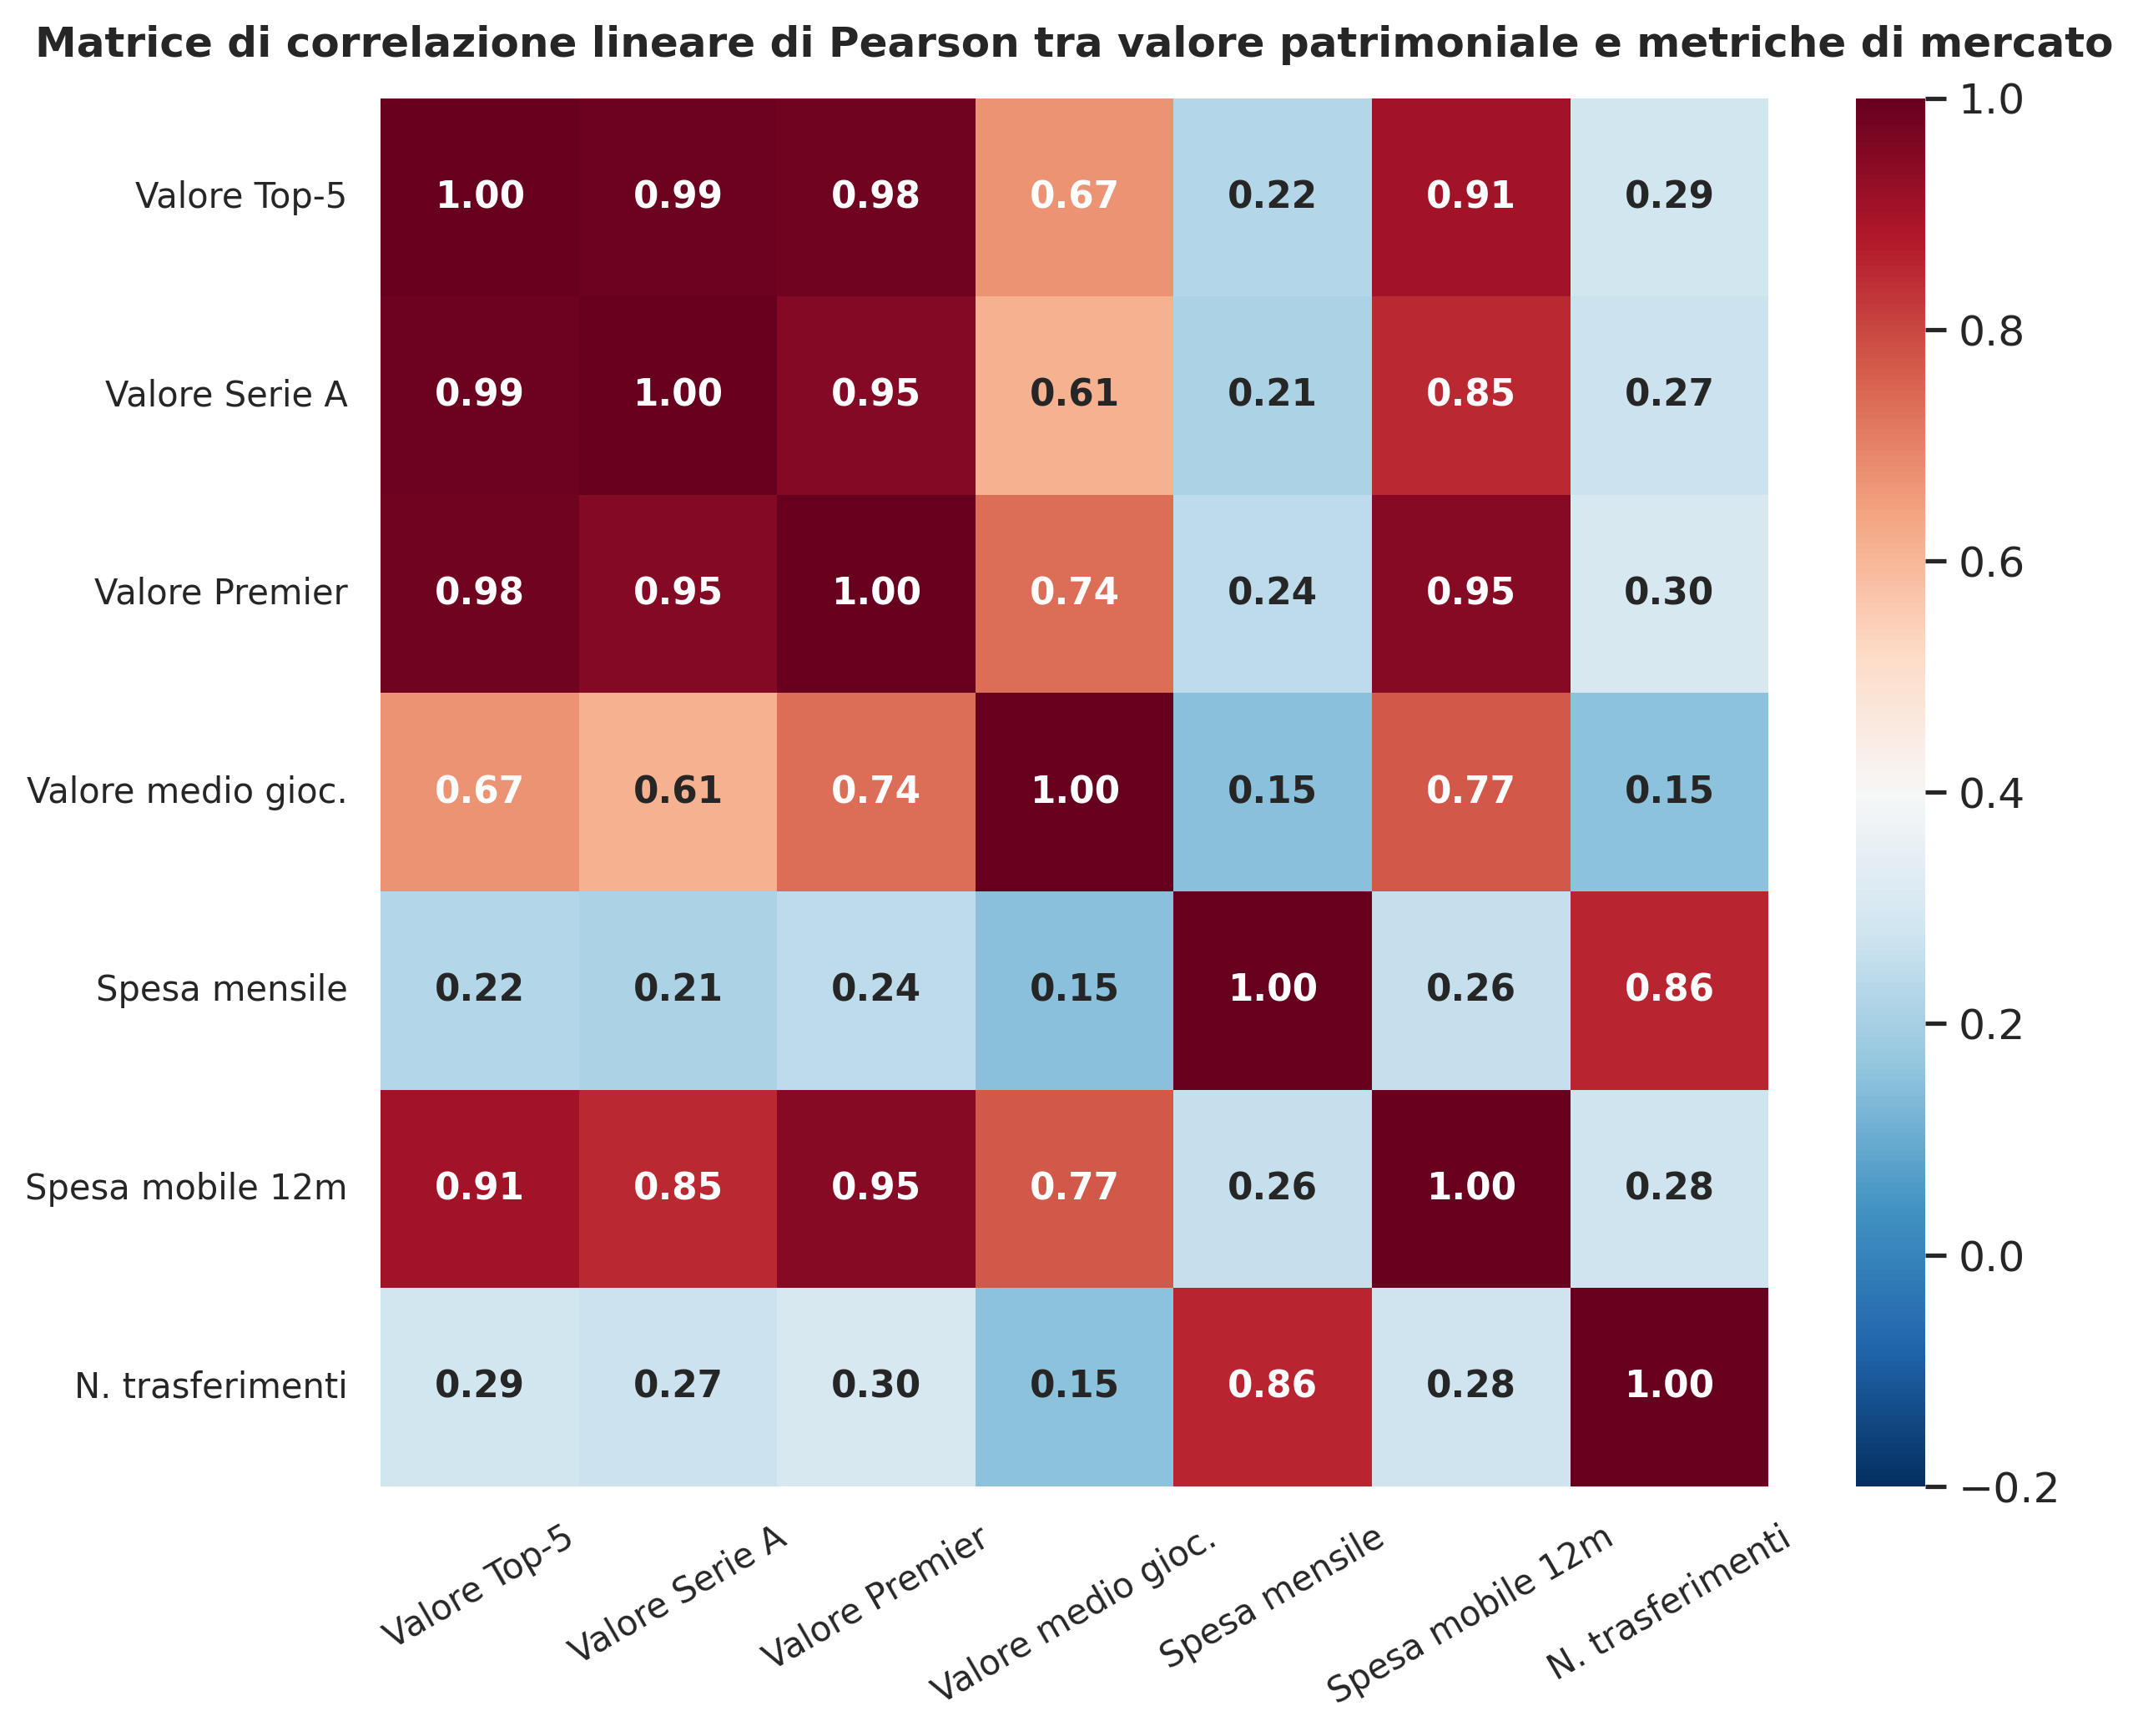
\includegraphics[width=0.85\textwidth]{capitolo7/img/fig11_eda_matrice_correlazione.png}
    \caption{Matrice di correlazione lineare di Pearson tra valore patrimoniale delle rose e metriche di spesa del calciomercato.}
    \label{fig:eda_matrice_corr}
\end{figure}

Dalla matrice di correlazione in Figura \ref{fig:eda_matrice_corr} emerge un'evidenza metodologica cruciale: la correlazione puntuale tra il valore delle rose e la spesa del singolo mese è pari a $r = 0,24$ (poiché la spesa si concentra in soli tre mesi mentre le rose mantengono valore tutto l'anno); tuttavia, non appena si considera la spesa cumulata mobile sui dodici mesi precedenti (\texttt{Spesa mobile 12m}), la correlazione con il valore aggregato Top-5 schizza a $r = 0,88$ ($r = 0,92$ con la Premier League e $r = 0,80$ con la Serie A). 

Tale risultato certifica che la liquidità immessa nel calciomercato durante l'anno costituisce la determinante economica primaria dell'inflazione del valore delle squadre, validando pienamente la scelta di impiegare la spesa e il numero di trasferimenti come predittori esogeni nei modelli SARIMAX del Capitolo 9.
